% !TeX root = thesis.tex
% !TeX spellcheck = en_US
% !TeX encoding = UTF-8
% !TeX program = xelatex
% TODO Change language to en_GB (recommended) or en_US for English documents
% \documentclass[11pt,a4paper,oneside]{report}             % Single-side
\documentclass[11pt,a4paper,twoside,openright]{report}  % Duplex

% thanks to http://tex.stackexchange.com/a/47579/71109
\usepackage{ifxetex}
\usepackage{ifluatex}
\newif\ifxetexorluatex % a new conditional starts as false
\ifnum 0\ifxetex 1\fi\ifluatex 1\fi>0
   \xetexorluatextrue
\fi

\ifxetexorluatex
  \usepackage{fontspec}
\else
  \usepackage[T1]{fontenc}
  \usepackage[utf8]{inputenc}
  \usepackage[lighttt]{lmodern}
\fi

\usepackage[english,magyar]{babel} % Alapértelmezés szerint utoljára definiált nyelv lesz aktív, de később külön beállítjuk az aktív nyelvet.

%\usepackage{cmap}
\usepackage{amsfonts,amsmath,amssymb} % Mathematical symbols.
%\usepackage[ruled,boxed,resetcount,linesnumbered]{algorithm2e} % For pseudocodes. % beware: this is not compatible with LuaLaTeX, see http://tex.stackexchange.com/questions/34814/lualatex-and-algorithm2e
\usepackage{booktabs} % For publication quality tables for LaTeX
\usepackage{graphicx}

%\usepackage{fancyhdr}
%\usepackage{lastpage}

\usepackage{anysize}
%\usepackage{sectsty}
\usepackage{setspace} % For setting line spacing

\usepackage[unicode]{hyperref} % For hyperlinks in the generated document.
\usepackage{xcolor}
\usepackage{listings} % For source code snippets.

\usepackage[amsmath,thmmarks]{ntheorem} % Theorem-like environments.

\usepackage[hang]{caption}

\singlespacing

\newcommand{\selecthungarian}{
	\selectlanguage{magyar}
	\setlength{\parindent}{2em}
	\setlength{\parskip}{0em}
	\frenchspacing
}

\newcommand{\selectenglish}{
	\selectlanguage{english}
	\setlength{\parindent}{0em}
	\setlength{\parskip}{0.5em}
	\nonfrenchspacing
	\renewcommand{\figureautorefname}{Figure}
	\renewcommand{\tableautorefname}{Table}
	\renewcommand{\partautorefname}{Part}
	\renewcommand{\chapterautorefname}{Chapter}
	\renewcommand{\sectionautorefname}{Section}
	\renewcommand{\subsectionautorefname}{Section}
	\renewcommand{\subsubsectionautorefname}{Section}
}

\usepackage[numbers]{natbib}
\usepackage{xspace}


\newcommand{\vikszerzoVezeteknev}{Gombos}
\newcommand{\vikszerzoKeresztnev}{Sándor Bence}

\newcommand{\vikkonzulensAMegszolitas}{}
\newcommand{\vikkonzulensAVezeteknev}{Schulcz}
\newcommand{\vikkonzulensAKeresztnev}{Róbert}

\newcommand{\vikkonzulensBMegszolitas}{}
\newcommand{\vikkonzulensBVezeteknev}{}
\newcommand{\vikkonzulensBKeresztnev}{}

\newcommand{\vikkonzulensCMegszolitas}{}
\newcommand{\vikkonzulensCVezeteknev}{}
\newcommand{\vikkonzulensCKeresztnev}{}

\newcommand{\vikcim}{Integrating open-source smart home software into a physical model} % Cím
\newcommand{\viktanszek}{\bmehit} % Tanszék
\newcommand{\vikdoktipus}{\bsc} % Dokumentum típusa (\bsc vagy \msc)
\newcommand{\vikmunkatipusat}{szakdolgozatot} % a "hallgató nyilatkozat" részhez: szakdolgozatot vagy diplomatervet

%--------------------------------------------------------------------------------------
% TDK-specifikus változók
%--------------------------------------------------------------------------------------
\newcommand{\tdkszerzoB}{Második Szerző} % Második szerző neve; hagyd üresen, ha egyedül írtad a TDK-t.
\newcommand{\tdkev}{2014} % A dolgozat írásának éve (pl. "2014") (Ez OTDK-nál eltérhet az aktuális évtől.)

% További adatok az OTDK címlaphoz (BME-s TDK-hoz nem kell kitölteni)
\newcommand{\tdkevfolyamA}{IV} % Első szerző évfolyama, római számmal (pl. IV).
\newcommand{\tdkevfolyamB}{III} % Második szerző évfolyama, római számmal (pl. III).
\newcommand{\tdkkonzulensbeosztasA}{egyetemi tanár} % Első konzulens beosztása (pl. egyetemi docens)
\newcommand{\tdkkonzulensbeosztasB}{doktorandusz} % Második konzulens beosztása (pl. egyetemi docens)

\newcommand{\szerzoMeta}{\vikszerzoVezeteknev{} \vikszerzoKeresztnev} % egy szerző esetén
%\newcommand{\szerzoMeta}{\vikszerzoVezeteknev{} \vikszerzoKeresztnev, \tdkszerzoB} % két szerző esetén

% Beállítások magyar nyelvű dolgozathoz
%%--------------------------------------------------------------------------------------
% Elnevezések
%--------------------------------------------------------------------------------------
\newcommand{\bme}{Budapesti Műszaki és Gazdaságtudományi Egyetem}
\newcommand{\vik}{Villamosmérnöki és Informatikai Kar}

\newcommand{\bmemit}{Méréstechnika és Információs Rendszerek Tanszék}

\newcommand{\keszitette}{Készítette}
\newcommand{\konzulens}{Konzulens}

\newcommand{\bsc}{Szakdolgozat}
\newcommand{\msc}{Diplomaterv}
\newcommand{\tdk}{TDK dolgozat}
\newcommand{\bsconlab}{BSc Önálló laboratórium}
\newcommand{\msconlabi}{MSc Önálló laboratórium 1.}
\newcommand{\msconlabii}{MSc Önálló laboratórium 2.}

\newcommand{\pelda}{Példa}
\newcommand{\definicio}{Definíció}
\newcommand{\tetel}{Tétel}

\newcommand{\bevezetes}{Bevezetés}
\newcommand{\koszonetnyilvanitas}{Köszönetnyilvánítás}
\newcommand{\fuggelek}{Függelék}

% Opcionálisan átnevezhető címek
%\addto\captionsmagyar{%
%\renewcommand{\listfigurename}{Saját ábrajegyzék cím}
%\renewcommand{\listtablename}{Saját táblázatjegyzék cím}
%\renewcommand{\bibname}{Saját irodalomjegyzék név}
%}

\newcommand{\szerzo}{\vikszerzoVezeteknev{} \vikszerzoKeresztnev}
\newcommand{\vikkonzulensA}{\vikkonzulensAMegszolitas\vikkonzulensAVezeteknev{} \vikkonzulensAKeresztnev}
\newcommand{\vikkonzulensB}{\vikkonzulensBMegszolitas\vikkonzulensBVezeteknev{} \vikkonzulensBKeresztnev}
\newcommand{\vikkonzulensC}{\vikkonzulensCMegszolitas\vikkonzulensCVezeteknev{} \vikkonzulensCKeresztnev}

\newcommand{\selectthesislanguage}{\selecthungarian}

\bibliographystyle{huplain}

\def\lstlistingname{lista}

\newcommand{\appendixnumber}{6}  % a fofejezet-szamlalo az angol ABC 6. betuje (F) lesz

% Settings for English documents
%--------------------------------------------------------------------------------------
% Elnevezések
%--------------------------------------------------------------------------------------
\newcommand{\bme}{Budapest University of Technology and Economics}
\newcommand{\vik}{Faculty of Electrical Engineering and Informatics}

\newcommand{\bmemit}{Department of Measurement and Information Systems}

\newcommand{\keszitette}{Author}
\newcommand{\konzulens}{Advisor}

\newcommand{\bsc}{Bachelor's Thesis}
\newcommand{\msc}{Master's Thesis}
\newcommand{\tdk}{Scientific Students' Association Report}
\newcommand{\bsconlab}{BSc Project Laboratory}
\newcommand{\msconlabi}{MSc Project Laboratory 1}
\newcommand{\msconlabii}{MSc Project Laboratory 2}

\newcommand{\pelda}{Example}
\newcommand{\definicio}{Definition}
\newcommand{\tetel}{Theorem}

\newcommand{\bevezetes}{Introduction}
\newcommand{\koszonetnyilvanitas}{Acknowledgements}
\newcommand{\fuggelek}{Appendix}

% Optional custom titles
%\addto\captionsenglish{%
%\renewcommand*{\listfigurename}{Your list of figures title}
%\renewcommand*{\listtablename}{Your list of tables title}
%\renewcommand*{\bibname}{Your bibliography title}
%}

\newcommand{\szerzo}{\vikszerzoKeresztnev{} \vikszerzoVezeteknev}
\newcommand{\vikkonzulensA}{\vikkonzulensAMegszolitas\vikkonzulensAKeresztnev{} \vikkonzulensAVezeteknev}
\newcommand{\vikkonzulensB}{\vikkonzulensBMegszolitas\vikkonzulensBKeresztnev{} \vikkonzulensBVezeteknev}
\newcommand{\vikkonzulensC}{\vikkonzulensCMegszolitas\vikkonzulensCKeresztnev{} \vikkonzulensCVezeteknev}

\newcommand{\selectthesislanguage}{\selectenglish}

\bibliographystyle{plainnat}

\newcommand{\ie}{i.e.\@\xspace}
\newcommand{\Ie}{I.e.\@\xspace}
\newcommand{\eg}{e.g.\@\xspace}
\newcommand{\Eg}{E.g.\@\xspace}
\newcommand{\etal}{et al.\@\xspace}
\newcommand{\etc}{etc.\@\xspace}
\newcommand{\vs}{vs.\@\xspace}
\newcommand{\viz}{viz.\@\xspace} % videlicet
\newcommand{\cf}{cf.\@\xspace} % confer
\newcommand{\Cf}{Cf.\@\xspace}
\newcommand{\wrt}{w.r.t.\@\xspace} % with respect to
\newcommand{\approximately}{approx.\@\xspace}

\newcommand{\appendixnumber}{1}  % a fofejezet-szamlalo az angol ABC 1. betuje (A) lesz



% \usepackage{parskip}
% \setlength{\parindent}{0pt} 
% \setlength{\parskip}{100pt}
% \addtolength{\parskip}{10pt}
% \renewcommand{\baselinestretch}{1.0}
% \everypar{\vspace{100pt}}

%--------------------------------------------------------------------------------------
% Page layout setup
%--------------------------------------------------------------------------------------
% we need to redefine the pagestyle plain
% another possibility is to use the body of this command without \fancypagestyle
% and use \pagestyle{fancy} but in that case the special pages
% (like the ToC, the References, and the Chapter pages)remain in plane style

\pagestyle{plain}
\marginsize{35mm}{25mm}{15mm}{15mm}

\setcounter{tocdepth}{3}
%\sectionfont{\large\upshape\bfseries}
\setcounter{secnumdepth}{3}

\sloppy % Margón túllógó sorok tiltása.
\widowpenalty=10000 \clubpenalty=10000 %A fattyú- és árvasorok elkerülése
\def\hyph{-\penalty0\hskip0pt\relax} % Kötőjeles szavak elválasztásának engedélyezése


%--------------------------------------------------------------------------------------
% Setup hyperref package
%--------------------------------------------------------------------------------------
\hypersetup{
    % bookmarks=true,            % show bookmarks bar?
    unicode=true,              % non-Latin characters in Acrobat's bookmarks
    pdftitle={\vikcim},        % title
    pdfauthor={\szerzoMeta},    % author
    pdfsubject={\vikdoktipus}, % subject of the document
    pdfcreator={\szerzoMeta},   % creator of the document
    pdfproducer={},    % producer of the document
    pdfkeywords={},    % list of keywords (separate then by comma)
    pdfnewwindow=true,         % links in new window
    colorlinks=true,           % false: boxed links; true: colored links
    linkcolor=black,           % color of internal links
    citecolor=black,           % color of links to bibliography
    filecolor=black,           % color of file links
    urlcolor=black             % color of external links
}


%--------------------------------------------------------------------------------------
% Set up listings
%--------------------------------------------------------------------------------------
\definecolor{lightgray}{rgb}{0.95,0.95,0.95}
\lstset{
	basicstyle=\scriptsize\ttfamily, % print whole listing small
	keywordstyle=\color{black}\bfseries, % bold black keywords
	identifierstyle=, % nothing happens
	% default behavior: comments in italic, to change use
	% commentstyle=\color{green}, % for e.g. green comments
	stringstyle=\scriptsize,
	showstringspaces=false, % no special string spaces
	aboveskip=3pt,
	belowskip=3pt,
	backgroundcolor=\color{lightgray},
	columns=flexible,
	keepspaces=true,
	escapeinside={(*@}{@*)},
	captionpos=b,
	breaklines=true,
	frame=single,
	float=!ht,
	tabsize=2,
	literate=*
		{á}{{\'a}}1	{é}{{\'e}}1	{í}{{\'i}}1	{ó}{{\'o}}1	{ö}{{\"o}}1	{ő}{{\H{o}}}1	{ú}{{\'u}}1	{ü}{{\"u}}1	{ű}{{\H{u}}}1
		{Á}{{\'A}}1	{É}{{\'E}}1	{Í}{{\'I}}1	{Ó}{{\'O}}1	{Ö}{{\"O}}1	{Ő}{{\H{O}}}1	{Ú}{{\'U}}1	{Ü}{{\"U}}1	{Ű}{{\H{U}}}1
}


%--------------------------------------------------------------------------------------
% Set up theorem-like environments
%--------------------------------------------------------------------------------------
% Using ntheorem package -- see http://www.math.washington.edu/tex-archive/macros/latex/contrib/ntheorem/ntheorem.pdf

\theoremstyle{plain}
\theoremseparator{.}
\newtheorem{example}{\pelda}

\theoremseparator{.}
%\theoremprework{\bigskip\hrule\medskip}
%\theorempostwork{\hrule\bigskip}
\theorembodyfont{\upshape}
\theoremsymbol{{\large \ensuremath{\centerdot}}}
\newtheorem{definition}{\definicio}

\theoremseparator{.}
%\theoremprework{\bigskip\hrule\medskip}
%\theorempostwork{\hrule\bigskip}
\newtheorem{theorem}{\tetel}


%--------------------------------------------------------------------------------------
% Some new commands and declarations
%--------------------------------------------------------------------------------------
\newcommand{\code}[1]{{\upshape\ttfamily\scriptsize\indent #1}}
\newcommand{\doi}[1]{DOI: \href{http://dx.doi.org/\detokenize{#1}}{\raggedright{\texttt{\detokenize{#1}}}}} % A hivatkozások közt így könnyebb DOI-t megadni.

\DeclareMathOperator*{\argmax}{arg\,max}
%\DeclareMathOperator*[1]{\floor}{arg\,max}
\DeclareMathOperator{\sign}{sgn}
\DeclareMathOperator{\rot}{rot}


%--------------------------------------------------------------------------------------
% Setup captions
%--------------------------------------------------------------------------------------
\captionsetup[figure]{
	width=.75\textwidth,
	aboveskip=10pt}

\renewcommand{\captionlabelfont}{\bf}
%\renewcommand{\captionfont}{\footnotesize\it}

%--------------------------------------------------------------------------------------
% Hyphenation exceptions
%--------------------------------------------------------------------------------------
\hyphenation{Shakes-peare Mar-seilles ár-víz-tű-rő tü-kör-fú-ró-gép}


\author{\vikszerzo}
\title{\viktitle}

%--------------------------------------------------------------------------------------
% Table of contents and the main text
%--------------------------------------------------------------------------------------
\begin{document}

\pagenumbering{gobble}

%TODO These includes define guidelines -- remove these
%~~~~~~~~~~~~~~~~~~~~~~~~~~~~~~~~~~~~~~~~~~~~~~~~~~~~~~~~~~~~~~~~~~~~~~~~~~~~~~~~~~~~~~
% \selecthungarian
%--------------------------------------------------------------------------------------
% Rovid formai es tartalmi tajekoztato
%--------------------------------------------------------------------------------------

\footnotesize
\begin{center}
\large
\textbf{\Large Általános információk, a diplomaterv szerkezete}\\
\end{center}

A diplomaterv szerkezete a BME Villamosmérnöki és Informatikai Karán:
\begin{enumerate}
\item	Diplomaterv feladatkiírás
\item	Címoldal
\item	Tartalomjegyzék
\item	A diplomatervező nyilatkozata az önálló munkáról és az elektronikus adatok kezeléséről
\item	Tartalmi összefoglaló magyarul és angolul
\item	Bevezetés: a feladat értelmezése, a tervezés célja, a feladat indokoltsága, a diplomaterv felépítésének rövid összefoglalása
\item	A feladatkiírás pontosítása és részletes elemzése
\item	Előzmények (irodalomkutatás, hasonló alkotások), az ezekből levonható következtetések
\item	A tervezés részletes leírása, a döntési lehetőségek értékelése és a választott megoldások indoklása
\item	A megtervezett műszaki alkotás értékelése, kritikai elemzése, továbbfejlesztési lehetőségek
\item	Esetleges köszönetnyilvánítások
\item	Részletes és pontos irodalomjegyzék
\item	Függelék(ek)
\end{enumerate}

Felhasználható a következő oldaltól kezdődő \LaTeX diplomatervsablon dokumentum tartalma. 

A diplomaterv szabványos méretű A4-es lapokra kerüljön. Az oldalak tükörmargóval készüljenek (mindenhol 2,5~cm, baloldalon 1~cm-es kötéssel). Az alapértelmezett betűkészlet a 12 pontos Times New Roman, másfeles sorközzel, de ettől kismértékben el lehet térni, ill. más betűtípus használata is megengedett.

Minden oldalon -- az első négy szerkezeti elem kivételével -- szerepelnie kell az oldalszámnak.

A fejezeteket decimális beosztással kell ellátni. Az ábrákat a megfelelő helyre be kell illeszteni, fejezetenként decimális számmal és kifejező címmel kell ellátni. A fejezeteket decimális aláosztással számozzuk, maximálisan 3 aláosztás mélységben (pl. 2.3.4.1.). Az ábrákat, táblázatokat és képleteket célszerű fejezetenként külön számozni (pl. 2.4. ábra, 4.2. táblázat vagy képletnél (3.2)). A fejezetcímeket igazítsuk balra, a normál szövegnél viszont használjunk sorkiegyenlítést. Az ábrákat, táblázatokat és a hozzájuk tartozó címet igazítsuk középre. A cím a jelölt rész alatt helyezkedjen el.

A képeket lehetőleg rajzoló programmal készítsék el, az egyenleteket egyenlet-szerkesztő segítségével írják le (A \LaTeX~ehhez kézenfekvő megoldásokat nyújt).

Az irodalomjegyzék szövegközi hivatkozása történhet sorszámozva (ez a preferált megoldás) vagy a Harvard-rendszerben (a szerző és az évszám megadásával). A teljes lista névsor szerinti sorrendben a szöveg végén szerepeljen (sorszámozott irodalmi hivatkozások esetén hivatkozási sorrendben). A szakirodalmi források címeit azonban mindig az eredeti nyelven kell megadni, esetleg zárójelben a fordítással. A listában szereplő valamennyi publikációra hivatkozni kell a szövegben (a \LaTeX-sablon a Bib\TeX~segítségével mindezt automatikusan kezeli). Minden publikáció a szerzők után a következő adatok szerepelnek: folyóirat cikkeknél a pontos cím, a folyóirat címe, évfolyam, szám, oldalszám tól-ig. A folyóiratok címét csak akkor rövidítsük, ha azok nagyon közismertek vagy nagyon hosszúak. Internetes hivatkozások megadásakor fontos, hogy az elérési út előtt megadjuk az oldal tulajdonosát és tartalmát (mivel a link egy idő után akár elérhetetlenné is válhat), valamint az elérés időpontját.

\vspace{5mm}
Fontos:
\begin{itemize}
	\item A szakdolgozatkészítő / diplomatervező nyilatkozata (a jelen sablonban szereplő szövegtartalommal) kötelező előírás, Karunkon ennek hiányában a szakdolgozat/diplomaterv nem bírálható és nem védhető!
	\item Mind a dolgozat, mind a melléklet maximálisan 15~MB méretű lehet!
\end{itemize}

\vspace{5mm}
\begin{center}
Jó munkát, sikeres szakdolgozatkészítést, ill. diplomatervezést kívánunk!
\end{center}

\normalsize
\selectthesislanguage

% %--------------------------------------------------------------------------------------
% Feladatkiiras (a tanszeken atveheto, kinyomtatott valtozat)
%--------------------------------------------------------------------------------------
\clearpage
\begin{center}
\large
\textbf{FELADATKIÍRÁS}\\
\end{center}

A feladatkiírást a tanszéki adminisztrációban lehet átvenni, és a leadott munkába eredeti, tanszéki pecséttel ellátott és a tanszékvezető által aláírt lapot kell belefűzni (ezen oldal \emph{helyett}, ez az oldal csak útmutatás). Az elektronikusan feltöltött dolgozatban már nem kell beleszerkeszteni ezt a feladatkiírást.


\selectthesislanguage

%~~~~~~~~~~~~~~~~~~~~~~~~~~~~~~~~~~~~~~~~~~~~~~~~~~~~~~~~~~~~~~~~~~~~~~~~~~~~~~~~~~~~~~
\hypersetup{pageanchor=false}
%--------------------------------------------------------------------------------------
%	The title page
%--------------------------------------------------------------------------------------
\begin{titlepage}
\begin{center}

\includegraphics[width=60mm,keepaspectratio]{figures/bme_logo.pdf}\\
\vspace{0.3cm}
\textbf{\bme}\\
\textmd{\vik}\\
\textmd{\viktanszek}\\[5cm]

\vspace{0.4cm}
{\huge \bfseries \vikcim}\\[0.8cm]
\vspace{0.5cm}
\textsc{\Large \vikdoktipus}\\[4cm]

{
	\renewcommand{\arraystretch}{0.85}
	\begin{tabular}{cc}
	 \makebox[7cm]{\emph{\keszitette}} & \makebox[7cm]{\emph{\konzulens}} \\ \noalign{\smallskip}
	 \makebox[7cm]{\szerzo} & \makebox[7cm]{\vikkonzulensA} \\
	  & \makebox[7cm]{\vikkonzulensB} \\
	  & \makebox[7cm]{\vikkonzulensC} \\
	\end{tabular}
}

\vfill
{\large \today}
\end{center}
\end{titlepage}
\hypersetup{pageanchor=false}

		   % Szakdolgozat/Diplomaterv címlap
%%% TDK címlap
\begin{titlepage}
  \begin{center}  
  
\includegraphics[width=7cm]{./figures/bme_logo.pdf}
  \vspace{0.3cm}
  
  \bme \\
  \vik \\
  \viktanszek \\
  \vspace{5cm}
  
  \huge {\vikcim}
  \vspace{1.5cm}
  
  \large {\textbf{\tdk}}
  \vfill
    
  {\Large 
  	\keszitette: \\ \vspace{0.3cm}
  	\szerzo \\
	\tdkszerzoB \\
  	\vspace{1.5cm}
  	\konzulens: \\ \vspace{0.3cm}
  	\vikkonzulensA \\
  	\vikkonzulensB \\
  }
  
  \vspace{2cm}
  \large {\tdkev}
 \end{center}
\end{titlepage}
%% Címlap vége
	% TDK címlap
%%% OTDK külső címlap
\begin{titlepage}
  	$\;$ 
	\vspace{5cm}
	
	\begin{center}
	\Huge
	\textbf{TDK-dolgozat}\let\thefootnote\relax\footnote{A dolgozat bemutatását a XXXXXXXXX  ``Lorem ipsum dolor sit amet'' című program támogatta.}
	\end{center}
	
	\vspace{13cm}
	
	\Large
	\hspace{8cm} \szerzo
	
	\hspace{8cm} \tdkszerzoB
	
	\hspace{8cm} \tdkev.
\end{titlepage}

\newpage
\thispagestyle{empty}


%% OTDK belső címlap
\begin{titlepage}
  \begin{center}  
  
\includegraphics[width=7cm]{./figures/bme_logo.pdf}
  \vspace{0.3cm}
  
  \bme \\
  \vik \\
  \viktanszek \\
  \vspace{3.5cm}
  
  \huge {\vikcim}
  \vspace{1.5cm}
  
  \large {\textbf{\vikdoktipus}}
  \vfill
    
  {\Large 
  	{\large \keszitette:} \\ \vspace{0.2cm}
  	\szerzo \\ \tdkevfolyamA. évfolyam \\
	\vspace{0.5cm}
	\tdkszerzoB \\ \tdkevfolyamB. évfolyam \\
  	\vspace{1.5cm}
  	{\large \konzulens:} \\ \vspace{0.2cm}
  	\vikkonzulensA,\\ \tdkkonzulensbeosztasA \\
  	\vspace{0.5cm}
  	\vikkonzulensB,\\ \tdkkonzulensbeosztasB \\
  }
  
  \vspace{2cm}
  \large {\tdkev.}
  
 \end{center}
\end{titlepage}   % OTDK címlap


% Table of Contents
%~~~~~~~~~~~~~~~~~~~~~~~~~~~~~~~~~~~~~~~~~~~~~~~~~~~~~~~~~~~~~~~~~~~~~~~~~~~~~~~~~~~~~~
\tableofcontents\vfill


% Declaration and Abstract
%~~~~~~~~~~~~~~~~~~~~~~~~~~~~~~~~~~~~~~~~~~~~~~~~~~~~~~~~~~~~~~~~~~~~~~~~~~~~~~~~~~~~~~
\selectlanguage{magyar}
\pagenumbering{gobble}
%--------------------------------------------------------------------------------------
% Nyilatkozat
%--------------------------------------------------------------------------------------
\begin{center}
\large
\textbf{HALLGATÓI NYILATKOZAT / STUDENT DECLARATION}\\
\end{center}

Alulírott \emph{\vikszerzoVezeteknev{} \vikszerzoKeresztnev}, szigorló hallgató kijelentem, hogy ezt a \vikmunkatipusat{} meg nem engedett segítség nélkül, saját magam készítettem, csak a megadott forrásokat (szakirodalom, eszközök stb.) használtam fel. Minden olyan részt, melyet szó szerint, vagy azonos értelemben, de átfogalmazva más forrásból átvettem, egyértelműen, a forrás megadásával megjelöltem.

Hozzájárulok, hogy a jelen munkám alapadatait (szerző(k), cím, angol és magyar nyelvű tartalmi kivonat, készítés éve, konzulens(ek) neve) a BME VIK nyilvánosan hozzáférhető elektronikus formában, a munka teljes szövegét pedig az egyetem belső hálózatán keresztül (vagy autentikált felhasználók számára) közzétegye. Kijelentem, hogy a benyújtott munka és annak elektronikus verziója megegyezik. Dékáni engedéllyel titkosított diplomatervek esetén a dolgozat szövege csak 3 év eltelte után válik hozzáférhetővé.
\break

\selectlanguage{english}
I, \emph{\vikszerzoKeresztnev{} \vikszerzoVezeteknev} hereby declare, that I have made this thesis myself, without the usage of unpermitted help and have only used sources (i.e. professional literature, tools etc.) noted in the bibliography. For every part, which I have used word by word or with the same meaning, but in different words, I made so with the clear and obvious marking of the source.

I agree, that BME VIK may publish my work's metainformation (author(s), title, English and Hungarian abstract, year of publication, name(s) of advisor(s)) in a publicly available, electronic manner and publish the full text content via the University's internal network (or for authenticated users). I declare, that the work turned in and its electronic version are the same. In the case of diploma thesis designs encrypted by the dean's permit, the content of the thesis may only be available 3 years later.

\selectlanguage{magyar}
\begin{flushleft}
\vspace*{1cm}
Budapest, \today
\end{flushleft}

\begin{flushright}
 \vspace*{1cm}
 \makebox[7cm]{\rule{6cm}{.4pt}}\\
 \makebox[7cm]{\emph{\vikszerzoVezeteknev{} \vikszerzoKeresztnev}}\\
 \makebox[7cm]{hallgató / student}
\end{flushright}
\thispagestyle{empty}

\vfill
\clearpage
\thispagestyle{empty} % an empty page

\selectthesislanguage

\pagenumbering{roman}
\setcounter{page}{1}

\selecthungarian

%----------------------------------------------------------------------------
% Abstract in Hungarian
%----------------------------------------------------------------------------
\chapter*{Kivonat}\addcontentsline{toc}{chapter}{Kivonat}

Az okosotthon rendszerek és otthon automatizálás technológia alapú megoldással nyújtanak kényelmi és egyéb szolgáltatásokat embereknek az otthoni környezetükben. Ez leginkább a ház "okos" eszközökkel (pl. villanykörték, hőmérséklet- és nedvességszenzorok, fűtési- és hűtési vezérlők) való felszerelését jelenti, hálózatba kötve egy vezérlő modullal, amit egy központi felhasználói felületen (általában egy okostelefonnal) lehet irányítani, akár a házon kívülről is. Ezek a rendszerek többek is lehetnek, mint egy kényelmi megoldás: növelhetik a ház energiahatékonyságát és bizonságát az erőforrások optimalizálásával, biztonsági felvételek analizálásával és egyéb módokon. Ez a szakdolgozat projekt bevezeti az olvasót az okosotthon rendszerek és otthon automatizálás világába, azoknak történelmébe, általános felépítésébe és kitér a piac vezető gyártóira, azoknak termékeire és megoldásaira. Ezt követően bemutatja egy fizikai demonstrációs modell tervezési és kivitelezési szakaszait, köztük a hardveres és szoftveres környezet kiválasztását. Végül bemutatja a demo modell használatát, felhasználási módjait és hiányosságait, továbbá a továbbfejlesztési lehetőségeket.

% A számítógépekkel vezérelt ipari rendszerek után az otthoni környezetben is felmerült ezeknek használata az otthonok energiatakarékosabbá és komfortosabbá tételéhez. Az ilyen rendszerekben a felhasználók a ház különböző rendszereit (pl. világítás, hűtés-fűtés, redőnyök) egy központosított felhasználói felületről vezérelhetik, valamint a mindennapi életet megkönnyítő automatizációkat állíthatnak be. A szakdolgozatomban bemutatom egy átlagos okosotthon rendszer felépítését, valamint elkészítek egy hasonló felépítésű, demonstrációs célú vezérelhető modellt és ennek a használati lehetőségeit kutatom. 
% \break
% % todo break fix, hogy ne ilyen magyar bekezdeses tragedia legyen

% Úgy vélem, hogy az okosotthon rendszerek használati lehetőségeinek kipróbálásához, egy valódi házban kialakított rendszer költséghatékony szimulálásához egy demonstrációs célú "doboz" modell megfelelőképpen alkalmas, ennek kialakítása során főképp két elvet követtem: a költséghatékonyságot (alacsony ár egy szakdolgozat projekthez) és a nyílt forráskódú szoftverek használatát. Manapság sajnos sokszor lehet hallani azt, hogy gyártók megszüntetik az egyébként nem annyira régi, még tökéletesen üzemelő termékeik támogatását, frissítését és ezzel sebezhetővé, nem működővé válnak, ami hozzájárul azok veszélyes hulladékká válásához. Ezt a problémát mérsékli az, ha valamilyen nyílt forráskódú szoftveres támogatás van azokra, mert a gyártás után évekkel később is friss szoftverrel tudnak üzemelni, illetve az általam kiválasztott hardverek később más projektekben is felhasználhatók. %todo forrás kivezetett termékre, pl. google nest secure
% \break

% A kereslet az okosotthon- és otthonautomatizációs technlólógiákra a megjelenésüktől kezdve folyamatosan növekedik, aktív piaci potenciál van bennük (a Világgazdasági Fórum (WEF) szerint 2030-ra elérheti a 13 billiót). Kezdetben főként csak egy kényelmi termékként gondoltak rájuk (például távolról való vezérelhetőség, egy központi felület), de emellé egyfajta megoldást adott a hatékonyságra és biztonságra is: előbbire például az automatizált fűtéssel, mozgásérzékelős lámpákkal, utóbbira a kamerákkal történő biztonsági felvételekkel, ennek elemzésével és a mozgáskorlátozottak támogatása.  %todo source from SHS article
\break

% A bevezető fejezetben szót ejtek az okosotthon megoldások történetéről, bemutatom egy átlagos okosotthon rendszer felépítését és a piacon elérhető elterjedtebb megoldásokat, valamint a témával való korábbi tapasztalataimról, motivációmról is írok. Az ezt követő tervezés fejezetben a demo modell tervezésével kapcsolatos előkészületeket mutatom be: annak általános céljait, követelményeit és elveit, továbbá a hardveres és szoftveres környezetek kiválasztását, annak indoklásait. A tervezést követően az elkészítés lépéseit mutatom be: a ház kialakítását, mikrokontrollerre történő eszközök bekötését, hálózat vitelét és ezeknek a szoftveres környezetének kialakítását. A modell elkészítését követően annak használatát mutatom be, értékelem az eredményeket és végül a továbbfejlesztési lehetőségeit ismertetem.


\vfill
\selectenglish


%----------------------------------------------------------------------------
% Abstract in English
%----------------------------------------------------------------------------
\chapter*{Abstract}\addcontentsline{toc}{chapter}{Abstract}

Smart home systems and home automation are technology based solutions for providing convenience and other services for people in their home environments. This is mostly in the form of a house fitted with "smart" devices (eg. lightbulbs, temperature and humidity sensors, heating and cooling actuators) networked with a controller module, which can be controlled via a user interface (generally via a smartphone), even remotely outside the house. These systems can be more, than a convenience solution: they can also increase the energy efficiency and safety of the house with resource usage optimization, analysis of security footage and other means. This thesis project introduces the reader to smart home systems and home automation, their history, general architecture and current market leading manufacturers, products and solutions. It is then followed by a presentation of a physical demonstrational model's planning and implementation phases, including the selection of hardware and software environments. Finally, showcases and evaluates the demo model's usage, use cases, shortcomings and provides opportunities of further development.

% After the usage of computer controlled systems in industrial installations, a demand for them appeared in home enviroments as well, in order to make homes more energy efficient and more comfortable to use. With these systems, users are able control different parts of their house (eg. lighting, cooling-heating, shutters) from a central user interface and set up automations to make their everyday life easier. In my thesis, I will be presenting the structure of a typical smart home system, furthermore create a physical model for demonstrational purposes and research its usage options.\break





% todo maybe summary of contents running text

\vfill
\selectthesislanguage

\newcounter{romanPage}
\setcounter{romanPage}{\value{page}}
\stepcounter{romanPage}



% The main part of the thesis
%~~~~~~~~~~~~~~~~~~~~~~~~~~~~~~~~~~~~~~~~~~~~~~~~~~~~~~~~~~~~~~~~~~~~~~~~~~~~~~~~~~~~~~
\pagenumbering{arabic}

%----------------------------------------------------------------------------
\chapter{\bevezetes}
%----------------------------------------------------------------------------

% A bevezető tartalmazza a diplomaterv-kiírás elemzését, történelmi előzményeit, a feladat indokoltságát (a motiváció leírását), az eddigi megoldásokat, és ennek tükrében a hallgató megoldásának összefoglalását.

% A bevezető szokás szerint a diplomaterv felépítésével záródik, azaz annak rövid leírásával, hogy melyik fejezet mivel foglalkozik.

In most conventional, "non-smart" houses or flats, utility and convenience devices (eg. lighting, heating, ventilation) are mostly controlled manually by hand via simple switches, knobs or the combination of the two, which requires people to be physically present at the scene to actuate them. In a home equipped with a smart home system, an extra computer and relay or transistor based system is added to them, which assists their actuation from centralized user interface (most often controlled on a smartphone application). Smart home systems can also be extended with digital sensors and other more fine tunable, convenience and security devices (in general just called as "smart" devices), such as temperature and humidity sensors, RGB lights, keycard readers, cameras. The sensors, along with other kinds of input (eg. time of the day, phone sensing) can be used to automate processes, which in turn would require manual interaction, such as turning on or off lights in rooms based on presence, rolling a shutter on or off at a certain time of a day. The general term for this process is called home automation, but this term also means the process of installation and usage a smart home system, so their meaning is almost identical in most contexts. \break

I believe that a demonstrational "box" model is an adequate and cost-effective solution to try out the usage of smart home systems and to simulate a proper system installed in a real house. During its implementation phase, I tried to follow two basic principles: cost-effectiveness (cheap price for a thesis project) and the usage of open-source software. We can often hear these days, that companies end supporting and updating their not so old, still completely functional products, which make them vulnerable to attacks and contributes to them becoming hazardous waste (take Amazon Echo Look as an example \cite{VergeAmazonEchoLook}). This problem can be mitigated to some extent with the usage of actively maintained open source software available to such devices, because this way they can run up-to-date software years after manufacturing, furthermore the devices chosen for the thesis project can be later repurposed in other projects.\break

The demand for smart home system and home automation technology has been steadily increasing since their inception and there is active market potential in them (the Worldwide Economic Forum predicts it could react 13 trillion dollars by 2030). Initially, they were considered only as a convenience product (with remote control, a centralized control interface), but since then they have also become a solution of efficiency and safety. Examples for the earlier are automatized heating and motion controlled lights, for the latter are recorded security footage and its analysis, support of handicapped people. \cite{ChakSHS}
% todo source

% todo sw is just as much important as hw?
% todo connection to iot

\section{Motivation, previous work}
My motivation behind choosing this thesis project was mostly my previous work on the topic and also that it combines more fields of expertise: various fields in Information Technology along with basic electronics.\break

For Training Project Laboratory, me and my two fellow students used an ESP-based microcontroller to control a few small electric components connected to it, which in large resembled a house's utilities. However, this was only a very rudimentary breadboard model, with continuous debug printing to the serial console and only a potentiometer and two buttons as inputs, but it was useful to familiarize ourselves with the usage and programming of a modern microcontroller liked by many hobby enthusiasts.\break

Throughout Project Laboratory, I took the project further and made a proper shoebox smart home system model. Along with a basic floorplan for various rooms and electronic components placed in them, it featured a web-controllable user interface. Its software architecture was comprised of three main components: a JavaScript backend responsible for maintaining the components' status and communication between the microcontroller and user, microcontroller code for controlling the electronic components (reading sensor data, setting output for actuators), receiving and sending data to the backend and finally a React-based frontend to send commands and receive readings to and from the backend. \break\break
%I decided to apply with it for Gadget Competition 2024 (organized by BME-MIT) and achieved 4th place on the competition.
% todo maybe pic of box and ui
For the Thesis Project, I've decided to continue work with the shoebox model, but focus more on the software side of improvement - the hardware, electronic components inside the box have remained mostly the same. I believe that the software of my Project Laboratory project was sufficient for showcasing simple smart home use cases in a demo environment, however would have been harder to further develop to extend with more devices and features than using already existing open-source smart home software with good community support, which I had also been looking forward to try out.

\section{A brief history of smart home systems, protocols}
% - development of protocols (not only used for smart homes) wifi, iot, zigbee, z-wave
% - cloud, subscription world and future, why local hosting is important

The Third Industrial Revolution's main innovation was the usage of IT and computer technology in order automate certain industrial processes and achieve a substantial speed up of tasks previously done via manual labor. \cite{UpkeepIndRev}
The appearance of Programmable Logic Controllers (PLCs) and innovation in Robotics made it easier, than ever to precisely control electric devices with a certain logic in industrial installations with much less human supervision. This aspect of computer-based electric and electronic device control is also important for the functioning of smart home systems, however the latter only started to be developed much more later, after a demand appeared for them and manufacturers started to experiment. %todo source

\subsection{Protocols}

The first major breakthrough, that helped the conception of the home automation field was the introduction of the X10 protocol and the devices utilizing it in the 1970s. X10 made it possible to control one lamp and one appliance via a remote control and a central control console by utilizing the house's already existing electrical wiring (on the same phase) to send commands from the control device the the appliances. Later versions of X10-based systems made it possible to control even more devices with more customization option and the platform still has some popularity among home automation enthusiasts, although it's mainly criticized for its lack of encryption. \cite{CavaX10}\break

However it took a while, before more sophisticated home automation solutions appeared, that utilized computers for controlling the apparatus and interfacing the users. One important aspect of such systems is the way devices communicate to each other, which also required a lot of research and development.
After the introduction of wired computer networking protocols, suchs as Ethernet, TCP/IP, which became the basis for the World Wide Web (WWW) in the early 90s, wireless computer and home automation related communication protocols and devices also appeared, but only later in the late 90s.
Although many automation devices could be networked via a UTP cable and utilize the aforementioned Ethernet and TCP/IP protocols, the development and usage of wireless protocols made their installation easier and contributed to their spread due to the lower cost of not having to run network cables all around the house besides the power cables and the possibility to make devices portable. IoT, or Internet of Devices is a collective term for the network of physical devices, vehicles, home appliances, and other embedded devices which connect to each other and exchange data. \cite{ShafiqIoTAttacks} Home automation devices make heavy use of IoT as well, besides other systems, such as smart grids, autonomous vehicles.\break

The first version of Wi-Fi was introduced in 1997 and made it possible for devices to comminicate wirelessly with a relatively high bandwidth of 2 Mbps on the 2.4Ghz ISM band, mainly designed as a Local Area Network (LAN) and Internet access protocol for home and office usage on laptops, PDAs and other mobile computers. Later versions improved bandwidth and some versions utilize the 5 and 6 GHz ISM bands instead for higher bandwidth - but at a lower range. \cite{IEEEWiFi}\break

Z-Wave, introduced in 1999 is a wireless communication protocol designed for residential and commercial building automation and utilizes the 900 MHz range for transmission, therefore achieves higher range at a lower bandwidth, still sufficient for the targeted kinds of devices, such as garage openers, smoke alarms and motions sensors. \cite{PCMagZWave}\break

Zigbee, an other low-power communication protocol was introduced in 2003 and originally used the 2.4 GHz ISM band (the 2023 Pro specification added 800-900 MHz support). It is mainly used in home automation, medical data collection, and industrial control systems.

Bluetooth is a short-range wireless protocol introduced in 1997, mainly used to wirelessly connect peripherals to mobile phones, desktops, and laptops and point-to-point mobile phone connection. \cite{IntelBluetooth} Some of the most common Bluetooth accessories include mice, keyboards, speakers, and headphones. It is less used in home automation, however can be useful in some situations, including detecting one's presence with their phone's transmitted Bluetooth signal.\break%todo maybe write more about BT, BTLE

Although wireless communication can be useful for many home automation related use cases, it might not always be the best solution opposed to a wired connection. A solution to ease the burden of wiring is Power over Ethernet (PoE), which was introduced in 2003. \cite{TTPoE} Power over Ethernet is a technology in wired Ethernet local area networks that enables the transmission of power necessary for every operating device to be carried on the same Ethernet cable, that is used for data transmission, therefore eliminates the need of a separate power cord running to the device. Devices, that make active use of it include VoIP phones, video surveillance cameras and high power LED lights. It requires the recipient device to have the necessary power converter electronics, that converts the higher voltage to the required device voltage and the source to be able to power it. If the source device (most likely a switch) it is connected to isn't PoE capable, it can still made so with the usage of a PoE adapter. For PoE, almost always a higher voltage is used than the recipient's internal because of less resistance for the same amount of power transmitted.\break

Smart home products really became popular in the 2010s, however with this came a problem among the many products by many manufacturers: they mostly used their own ecosystem, on top of certain standard protocols and this made their cooperation hard, users had to use different interfaces and ecosystems for each owned device. A proposed solution to allow products from different manufacturers to securely communicate in a standardized manner is Matter. \cite{PCMagMatter} The working group behind it was formed in 2019 by Amazon, Apple, Google and other big corporations, and it's being actively developed and adapted by many manufacturers for more and more types of appliances. It is based on the Internet Protocol and uses other existing protocols for the underlying connections, such as Wi-Fi and Bluetooth.
%todo maybe thread, mqtt

\subsection{Solutions}
In the mid 2000s, companies with a strong focus on home automation products started appearing, such as Control4 in 2004, Insteon and Savant in 2005. \cite{Control4about} \cite{WPInsteonFirstLook} \cite{SavantCompInfo}\break
Later in the early 2010s, many big IT corporations also jumped onto the hype around smart home systems and released products on the market, often bundled with their voice assistant solutions. This was also helped by the spread of smartphones after the introduction of early iPhone and Android phones and tablets at the end of the earlier decade. Manufacturers could use their software platform to build applications for interfacing users and it also meant that they could make their systems cheaper by only optionally including a control console device as that could be substituted by the phones or tablets. Such platforms include Amazon's Alexa Smart Home with their Alexa voice assistant and Echo smart speakers, Google's Home with their Nest devices and Assistant voice assistant, Apple's HomeKit software platform. \cite{AmazonAlexaSH} \cite{GoogleHome} \cite{GoogleAssistant} \cite{AppleHome}\break

A typical smart home system usually includes smart devices, that mostly provide or control home utilities, along with detectors, sensors and other devices facilitating extra services (eg. voice assistant). Smart utility devices mostly replace their conventional equivalent (which aren't "smart"), their retrofitting isn't hard. Such utility devices comprise of controllable monochrome or RGB LED lightbulbs and light strips, thermostats for heating and cooling (A/C)
% todo better source than energybot

In the 2010s, cloud computing technology also started started to get traction, as big IT corporations launched theirs, take Amazon Web Services (AWS), Google Cloud Platform (GCP) and Microsoft Azure as examples. Cloud computing means that such providers provide on-demand delivery of IT resources over the Internet, so that that companies can use this to outsource different portions of their infrastructure instead of having to operate everything themselves. \cite{AWScloud} It can lead to significant cost savings besides the more agile and faster deployments, scaling of resources according to demand. This technology was also beneficial for smart home solutions, for a number of reasons. \cite{ChakSHS} Most modern smart home devices require some form of background IT infrastructure (eg. control server) for management, remote access and data collection, which is something that most customers aren't tech savvy enough to set up themselves and operate, regularly update. The amount of data generated also varies device-by-device, typically security cameras would require the most amount of data to be stored somewhere. For these use cases, many manufacturers use cloud services because of their advantages against a locally hosted environment.\break

double edged sword
corpos wanting to get their hand on data
privacy


why local hosting is also important
privacy, internet outage
(fb's lockout 2021)

mention home assistant

\section{Architecture and devices of a typical smart home system}

Every smart home system solution and product is different, however there are a few key concepts and parts, that most solutions follow and share. In this thesis, a typical IoT-based smart home system's architecture and devices are presented with some variations, along with the general concepts that they follow. There are also smart home systems which utilize Artificial Intelligence (AI) and its forms in Machine Learning (ML), Deep Learning (DL) and Neutral Networks (NN), furthermore Multiagent System (MAS) and Image Processing (IP) based smart home systems, however these aren't going to be covered in the thesis due to them being not used in the accomplished physical demo model presented in the upcoming chapters. \cite{ChakSHS}\break

% todo draw.io diagram of a shs

Many IoT-based smart home systems use a controller as a brains of operations, although its form of implementation can vary to a great extent based on the platform. One form of implementation is a controller "box" or "hub", where a physical device is present, which manages the appliances, collects data and stores it for later review and provides an interface (on the devices itself, or from a smartphone or computer application) for user control.
todo cloud or self hosted, double edged sword, privacy etc
network

- devices:
sensors
actuators
light



- user interface
controlled from central console
smartphone, tablet app
web interface

remote access solution: nat, mqtt

- etc, tadada

% \section{Current solutions of the market}
% - products

% - alexa, google voice, etc voice assistants

% %----------------------------------------------------------------------------
\chapter{\LaTeX-eszközök}
\label{sec:LatexTools}
%----------------------------------------------------------------------------
\section{A szerkesztéshez használatos eszközök}
%----------------------------------------------------------------------------
Ez a sablon TeXstudio 2.8.8 szerkesztővel készült. A TeXstudio egy platformfüggetlen, Windows, Linux és Mac OS alatt is elérhető \LaTeX-szerkesztőprogram számtalan hasznos szolgáltatással (\refstruc{fig:TeXstudio}). A szoftver ingyenesen letölthető\footnote{A TeXstudio hivatalos oldala: \url{http://texstudio.sourceforge.net/}}.

\begin{figure}[!ht]
\centering
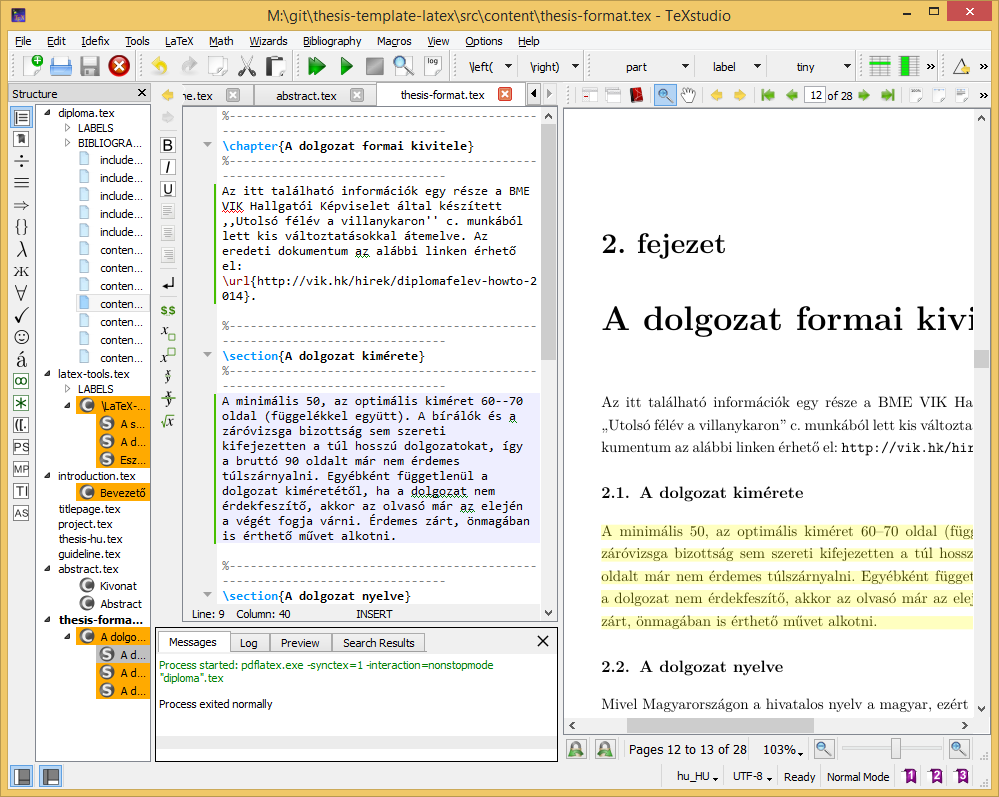
\includegraphics[width=150mm, keepaspectratio]{figures/TeXstudio.png}
\caption{A TeXstudio \LaTeX-szerkesztő.}
\label{fig:TeXstudio}
\end{figure}

A TeXstudio telepítése után érdemes még letölteni a magyar nyelvű helyesírásellenőrző-szótárakat hozzá. A TeXstudio az OpenOffice-hoz használatos formátumot tudja kezelni. A TeXstudio beállításainál a \verb+General+ fülön a \verb+Dictionaries+ résznél tudjuk megadni, hogy melyik szótárat használja.

Egy másik használható Windows alapú szerkesztőprogram a LEd\footnote{A LEd hivatalos oldala: \url{http://www.latexeditor.org/}} (LaTeX Editor), a TeXstudio azonban stabilabb, gyorsabb, és jobban használható.

%----------------------------------------------------------------------------
\section{A dokumentum lefordítása Windows alatt}
%----------------------------------------------------------------------------
A TeXstudio és a LEd kizárólag szerkesztőprogram (bár az utóbbiban DVI-nézegető is van), így a dokumentum fordításához szükséges eszközöket nem tartalmazza. Windows alatt alapvetően két lehetőség közül érdemes választani: MiKTeX (\url{http://miktex.org/}) és TeX Live (\url{http://www.tug.org/texlive/}) programcsomag. Az utóbbi működik Mac OS X, GNU/Linux alatt és Unix-származékokon is. A MiKTeX egy alapcsomag telepítése után mindig letölti a használt funkciókhoz szükséges, de lokálisan hiányzó \TeX-csomagokat, míg a TeX Live DVD ISO verzóban férhető hozzá. Ez a dokumentum TeX Live 2008 programcsomag segítségével fordult, amelynek DVD ISO verziója a megadott oldalról letölthető. A sablon lefordításához a disztribúcióban szereplő \verb+magyar.ldf+ fájlt a \verb+http://www.math.bme.hu/latex/+ változatra kell cserélni, vagy az utóbbi változatot be kell másolni a projekt-könyvtárba (ahogy ezt meg is tettük a sablonban) különben anomáliák tapasztalhatók a dokumentumban (pl. az ábra- és táblázat-aláírások formátuma nem a beállított lesz, vagy bizonyos oldalakon megjelenik alapértelmezésben egy fejléc). A TeX Live 2008-at még nem kell külön telepíteni a gépre, elegendő DVD-ről (vagy az ISO fájlból közvetlenül, pl. DaemonTools-szal) használni.

Ha a MiKTeX csomagot használjuk, akkor parancssorból a következő módon tudjuk újrafordítani a teljes dokumentumot:

\begin{lstlisting}[language=bash,frame=single,float=!ht]
$ texify -p thesis.tex
\end{lstlisting}

A \verb+texify+ parancs a MiKTex programcsomag \verb+miktex/bin+ alkönyvtárában található. A parancs gondoskodik arról, hogy a szükséges lépéseket (fordítás, hivatkozások generálása stb.) a megfelelő sorrendben elvégezze. A \verb+-p+ kapcsoló hatására PDF-et generál. A fordítást és az ideiglenes fájlok törlését elvégezhetjük a sablonhoz mellékelt \verb+manual_build.bat+ szkript segítségével is.

A \TeX-eszközöket tartalmazó programcsomag binárisainak elérési útját gyakran be kell állítani a szerkesztőprogramban, például TeXstudio esetén legegyszerűbben az \verb+Options / Configure TeXstudio... / Commands+ menüponttal előhívott dialógusablakban tehetjük ezt meg.

A PDF-\LaTeX~használata esetén a generált dokumentum közvetlenül PDF-formátumban áll rendelkezésre. Amennyiben a PDF-fájl egy PDF-nézőben (pl. Adobe Acrobat Reader vagy Foxit PDF Reader) meg van nyitva, akkor a fájlleírót a PDF-néző program tipikusan lefoglalja. Ilyen esetben a dokumentum újrafordítása hibaüzenettel kilép. Ha bezárjuk és újra megnyitjuk a PDF dokumentumot, akkor pedig a PDF-nézők többsége az első oldalon nyitja meg a dokumentumot, nem a legutóbb olvasott oldalon. Ezzel szemben például az egyszerű és ingyenes \textcolor{blue}{Sumatra PDF} nevű program képes arra, hogy a megnyitott dokumentum megváltozását detektálja, és frissítse a nézetet az aktuális oldal megtartásával.

%----------------------------------------------------------------------------
\section{Eszközök Linuxhoz}
%----------------------------------------------------------------------------
Linux operációs rendszer alatt is rengeteg szerkesztőprogram van, pl. a KDE alapú Kile jól használható. Ez ingyenesen letölthető, vagy éppenséggel az adott Linux-disztribúció eleve tartalmazza, ahogyan a dokumentum fordításához szükséges csomagokat is. Az Ubuntu Linux disztribúciók alatt például legtöbbször a \verb+texlive-*+ csomagok telepítésével használhatók a \LaTeX-eszközök. A jelen sablon fordításához szükséges csomagok (kb. 0,5 GB) az alábbi paranccsal telepíthetők:

\begin{lstlisting}[language=bash,morekeywords={sudo,apt\-get},alsoletter={-},breaklines=true]
$ sudo apt-get install texlive-latex-extra texlive-fonts-extra texlive-fonts-recommended texlive-xetex texlive-science
\end{lstlisting}

Amennyiben egy újabb csomag hozzáadása után hiányzó fájlra utaló hibát kapunk a fordítótól, telepítenünk kell az azt tartalmazó TeX Live csomagot. Ha pl. a \verb+bibentry+ csomagot szeretnénk használni, futtassuk az alábbi parancsot:

\begin{lstlisting}[language=bash,morekeywords={apt\-cache},alsoletter={-},breaklines=true]
$ apt-cache search bibentry
texlive-luatex - TeX Live: LuaTeX packages
\end{lstlisting}

Majd telepítsük fel a megfelelő TeX Live csomagot, jelen esetben a `texlive-lualatex`-et. (Egy LaTeX csomag több TeX Live csomagban is szerepelhet.)

Ha gyakran szerkesztünk más \LaTeX dokumentumokat is, kényelmes és biztos megoldás a teljes TeX Live disztribúció telepítése, ez azonban kb. 4 GB helyet igényel.

\begin{lstlisting}[language=bash,morekeywords={sudo,apt\-get},alsoletter={-},breaklines=true]
sudo apt-get install texlive-full
\end{lstlisting}

% %----------------------------------------------------------------------------
\chapter{A dolgozat formai kivitele}
%----------------------------------------------------------------------------
Az itt található információk egy része a BME VIK Hallgatói Képviselet által készített ,,Utolsó félév a villanykaron'' c. munkából lett kis változtatásokkal átemelve. Az eredeti dokumentum az alábbi linken érhető el: \url{http://vik.hk/hirek/diplomafelev-howto-2015}.

%----------------------------------------------------------------------------
\section{A dolgozat kimérete}
%----------------------------------------------------------------------------
Szakdolgozat esetében minimum 30, 45 körüli ajánlott oldalszám lehet az iránymutató. De mindenképp érdemes rákérdezni a konzulensnél is az elvárásokra, mert tanszékenként változóak lehetnek az elvárások.

Mesterképzésen a Diplomatervezés 1 esetében a beszámoló még inkább az Önálló laboratóriumi beszámolókhoz hasonlít, tanszékenként eltérő formai követelményekkel, -- egy legalább 30 oldal körüli dolgozat az elvárt -- és az elmúlt fél éves munkáról szól. De egyben célszerű, ha ez a végleges diplomaterv alapja is. (A végleges 60-90 oldal körülbelül a hasznos részre nézve)


%----------------------------------------------------------------------------
\section{A dolgozat nyelve}
%----------------------------------------------------------------------------
Mivel Magyarországon a hivatalos nyelv a magyar, ezért alapértelmezésben magyarul kell megírni a dolgozatot. Aki külföldi posztgraduális képzésben akar részt venni, nemzetközi szintű tudományos kutatást szeretne végezni, vagy multinacionális cégnél akar elhelyezkedni, annak célszerű angolul megírnia diplomadolgozatát. Mielőtt a hallgató az angol nyelvű verzió mellett dönt, erősen ajánlott mérlegelni, hogy ez mennyi többletmunkát fog a hallgatónak jelenteni fogalmazás és nyelvhelyesség terén, valamint -- nem utolsó sorban -- hogy ez mennyi többletmunkát fog jelenteni a konzulens illetve bíráló számára. Egy nehezen olvasható, netalán érthetetlen szöveg teher minden játékos számára.

%----------------------------------------------------------------------------
\section{A dokumentum nyomdatechnikai kivitele}
%----------------------------------------------------------------------------
A dolgozatot A4-es fehér lapra nyomtatva, 2,5 centiméteres margóval (+1~cm kötésbeni), 11--12 pontos betűmérettel, talpas betűtípussal és másfeles sorközzel célszerű elkészíteni.

Annak érdekében, hogy a dolgozat külsőleg is igényes munka benyomását keltse, érdemes figyelni az alapvető tipográfiai szabályok betartására~\cite{Jeney}.

% % !TeX spellcheck = hu_HU
% !TeX encoding = UTF-8
% !TeX program = xelatex
%----------------------------------------------------------------------------
\chapter{A \LaTeX-sablon használata}
%----------------------------------------------------------------------------

Ebben a fejezetben röviden, implicit módon bemutatjuk a sablon használatának módját, ami azt jelenti, hogy sablon használata ennek a dokumentumnak a forráskódját tanulmányozva válik teljesen világossá. Amennyiben a szoftver-keretrendszer telepítve van, a sablon alkalmazása és a dolgozat szerkesztése \LaTeX-ben a sablon segítségével tapasztalataink szerint jóval hatékonyabb, mint egy WYSWYG (\emph{What You See is What You Get}) típusú szövegszerkesztő esetén (pl. Microsoft Word, OpenOffice).

%----------------------------------------------------------------------------
\section{Címkék és hivatkozások}
%----------------------------------------------------------------------------
A \LaTeX~dokumentumban címkéket (\verb+\label+) rendelhetünk ábrákhoz, táblázatokhoz, fejezetekhez, listákhoz, képletekhez stb. Ezekre a dokumentum bármely részében hivatkozhatunk, a hivatkozások automatikusan feloldásra kerülnek.

A sablonban makrókat definiáltunk a hivatkozások megkönnyítéséhez. Ennek megfelelően minden ábra (\emph{figure}) címkéje \verb+fig:+ kulcsszóval kezdődik, míg minden táblázat (\emph{table}), képlet (\emph{equation}), fejezet (\emph{section}) és lista (\emph{listing}) rendre a \verb+tab:+, \verb+eq:+, \verb+sec:+ és \verb+lst:+ kulcsszóval kezdődik, és a kulcsszavak után tetszőlegesen választott címke használható. Ha ezt a konvenciót betartjuk, akkor az előbbi objektumok számára rendre a \verb+\figref+, \verb+\tabref+, \verb+\eqref+, \verb+\sectref+ és \verb+\listref+ makrókkal hivatkozhatunk. A makrók paramétere a címke, amelyre hivatkozunk (a kulcsszó nélkül). Az összes említett hivatkozástípus, beleértve az \verb+\url+ kulcsszóval bevezetett web-hivatkozásokat is a  \verb+hyperref+\footnote{Segítségével a dokumentumban megjelenő hivatkozások nem csak dinamikussá válnak, de színezhetők is, bővebbet erről a csomag dokumentációjában találunk. Ez egyúttal egy példa lábjegyzet írására.} csomagnak köszönhetően aktívak a legtöbb PDF-nézegetőben, rájuk kattintva a dokumentum megfelelő oldalára ugrik a PDF-néző vagy a megfelelő linket megnyitja az alapértelmezett böngészővel. A \verb+hyperref+ csomag a kimeneti PDF-dokumentumba könyvjelzőket is készít a tartalomjegyzékből. Ez egy szintén aktív tartalomjegyzék, amelynek elemeire kattintva a nézegető behozza a kiválasztott fejezetet.

%----------------------------------------------------------------------------
\section{Ábrák és táblázatok}
%----------------------------------------------------------------------------
Használjunk vektorgrafikus ábrákat, ha van rá módunk. PDFLaTeX használata esetén PDF formátumú ábrákat lehet beilleszteni könnyen, az EPS (PostScript) vektorgrafikus képformátum beillesztését a PDFLaTeX közvetlenül nem támogatja (de lehet konvertálni, lásd később). Ha vektorgrafikus formában nem áll rendelkezésünkre az ábra, akkor a  veszteségmentes PNG, valamint a veszteséges JPEG formátumban érdemes elmenteni.  Figyeljünk arra, hogy ilyenkor a képek felbontása elég nagy legyen ahhoz, hogy nyomtatásban is megfelelő minőséget nyújtson (legalább 300 dpi javasolt). A dokumentumban felhasznált képfájlokat a dokumentum forrása mellett érdemes tartani, archiválni, mivel ezek hiányában a dokumentum nem fordul újra. Ha lehet, a vektorgrafikus képeket vektorgrafikus formátumban is érdemes elmenteni az újrafelhasználhatóság (az átszerkeszthetőség) érdekében.

Kapcsolási rajzok legtöbbször kimásolhatók egy vektorgrafikus programba (pl. CorelDraw) és onnan nagyobb felbontással raszterizálva kimenthatők PNG formátumban. Ugyanakkor kiváló ábrák készíthetők Microsoft Visio vagy hasonló program használatával is: Visio-ból az ábrák közvetlenül PDF-be is menthetők.

Lehetőségeink Matlab ábrák esetén:
\begin{itemize}
	\item Képernyőlopás (\emph{screenshot}) is elfogadható minőségű lehet a dokumentumban, de általában jobb felbontást is el lehet érni más módszerrel.
	\item A Matlab ábrát a \verb+File/Save As+ opcióval lementhetjük PNG formátumban (ugyanaz itt is érvényes, mint korábban, ezért nem javasoljuk).
	\item A Matlab ábrát az \verb+Edit/Copy figure+ opcióval kimásolhatjuk egy vektorgrafikus programba is és onnan nagyobb felbontással raszterizálva kimenthatjük PNG formátumban (nem javasolt).
	\item Javasolt megoldás: az ábrát a \verb+File/Save As+ opcióval EPS \emph{vektorgrafikus} formátumban elmentjük, PDF-be konvertálva beillesztjük a dolgozatba.
\end{itemize}
Az EPS kép az \verb+epstopdf+ programmal\footnote{a korábban említett \LaTeX-disztribúciókban megtalálható} konvertálható PDF formátumba. Célszerű egy batch-fájlt készíteni az összes EPS ábra lefordítására az alábbi módon (ez Windows alatt működik).
\begin{lstlisting}[language=]
@echo off
for %%j in (*.eps) do (
  echo converting file "%%j"
  epstopdf "%%j"
)
echo done .
\end{lstlisting}

Egy ilyen parancsfájlt (\verb+convert.cmd+) elhelyeztük a sablon \verb+figures\eps+ könyvtárába, így a felhasználónak csak annyi a dolga, hogy a \verb+figures\eps+ könyvtárba kimenti az EPS formátumú vektorgrafikus képet, majd lefuttatja a \verb+convert.cmd+ parancsfájlt, ami PDF-be konvertálja az EPS fájlt.

Ezek után a PDF-ábrát ugyanúgy lehet a dokumentumba beilleszteni, mint a PNG-t vagy a JPEG-et. A megoldás előnye, hogy a lefordított dokumentumban is vektorgrafikusan tárolódik az ábra, így a mérete jóval kisebb, mintha raszterizáltuk volna beillesztés előtt. Ez a módszer minden -- az EPS formátumot ismerő -- vektorgrafikus program (pl. CorelDraw) esetén is használható.

A képek beillesztésére \az+\refstruc{sec:LatexTools}ben mutattunk be példát (\refstruc{fig:TeXstudio}). Az előző mondatban egyúttal az automatikusan feloldódó ábrahivatkozásra is láthatunk példát. Több képfájlt is beilleszthetünk egyetlen ábrába. Az egyes képek közötti horizontális és vertikális margót metrikusan szabályozhatjuk (\refstruc{fig:HVSpaces}). Az ábrák elhelyezését számtalan tipográfiai szabály egyidejű teljesítésével a fordító maga végzi, a dokumentum írója csak preferenciáit jelezheti a fordító felé (olykor ez bosszúságot is okozhat, ilyenkor pl. a kép méretével lehet játszani).

\begin{figure}[!ht]
	\centering
	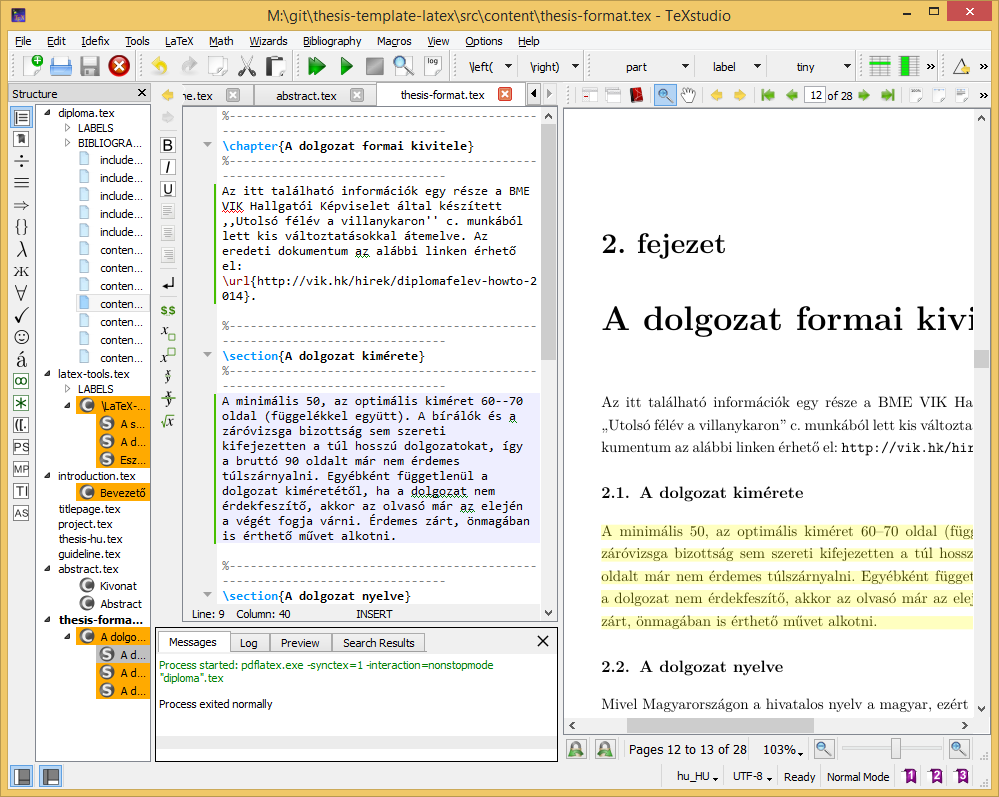
\includegraphics[width=67mm, keepaspectratio]{figures/TeXstudio.png}\hspace{1cm}
	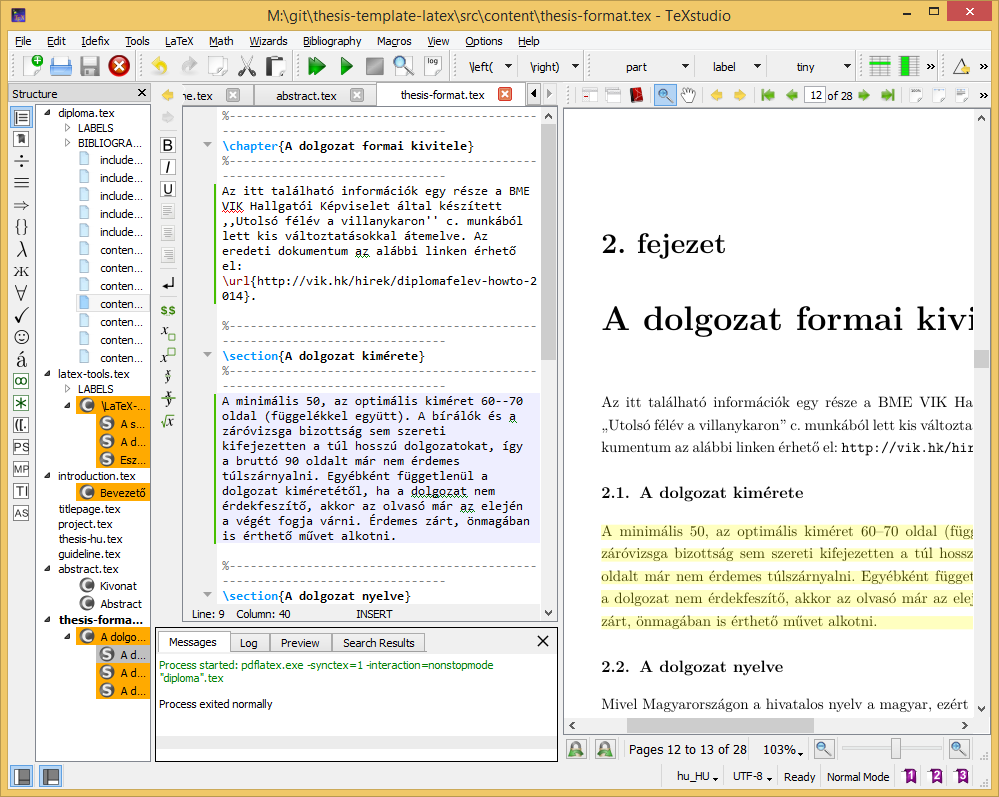
\includegraphics[width=67mm, keepaspectratio]{figures/TeXstudio.png}\\\vspace{5mm}
	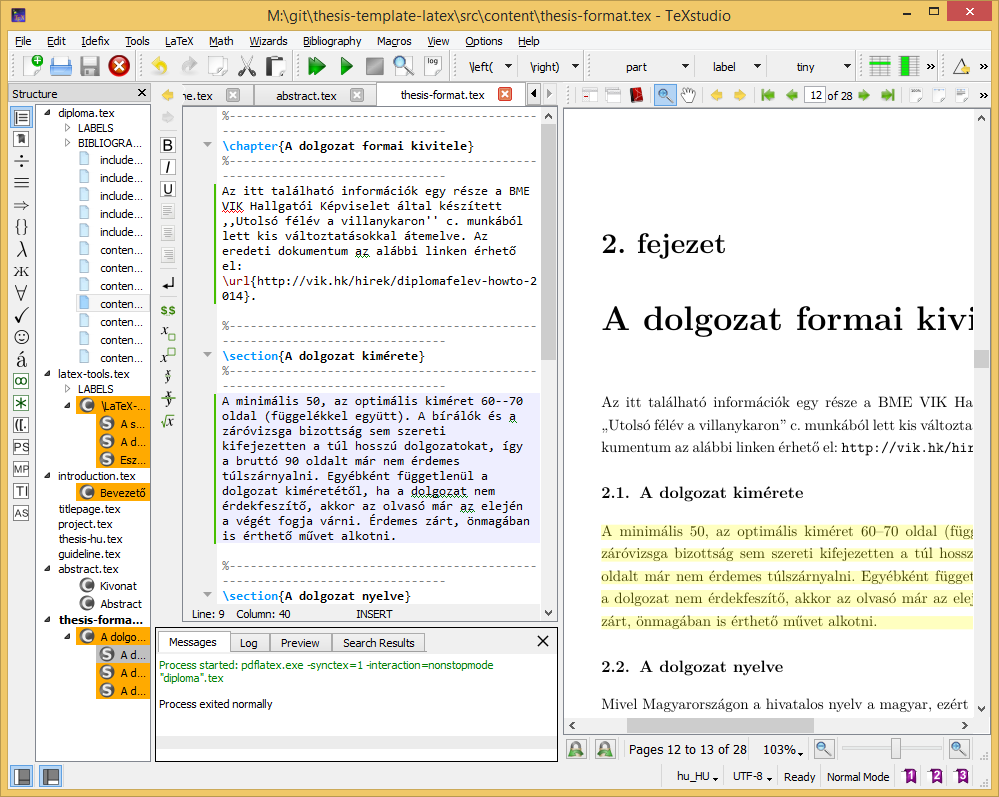
\includegraphics[width=67mm, keepaspectratio]{figures/TeXstudio.png}\hspace{1cm}
	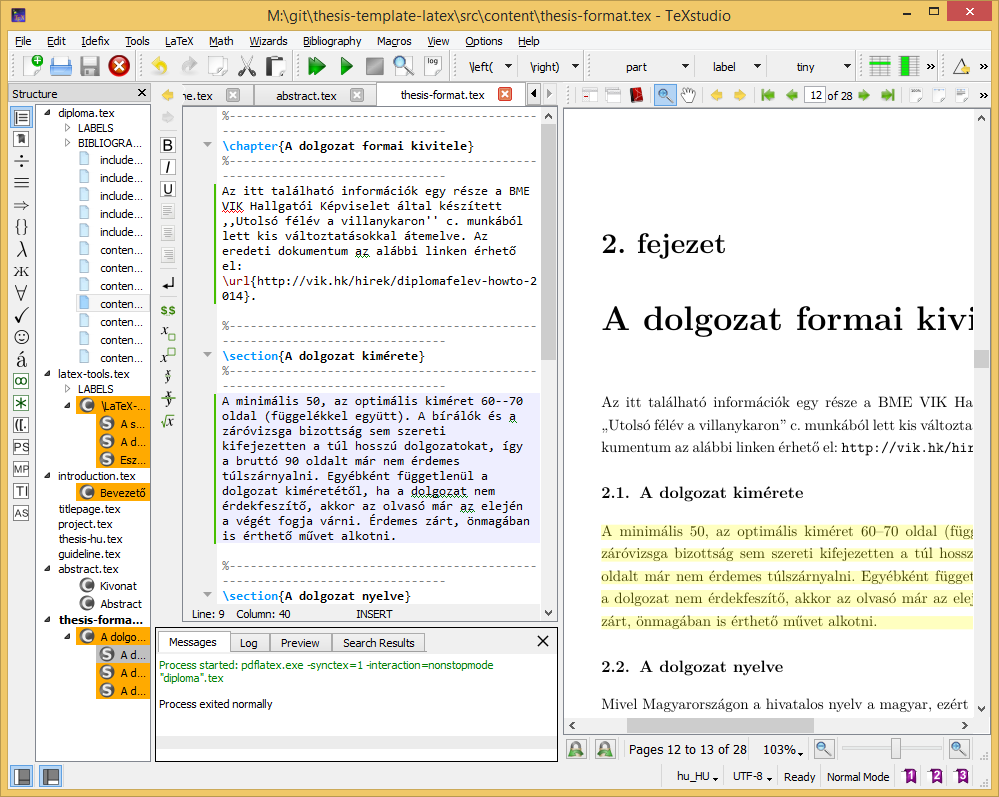
\includegraphics[width=67mm, keepaspectratio]{figures/TeXstudio.png}
	\caption{Több képfájl beillesztése esetén térközöket is érdemes használni.}
	\label{fig:HVSpaces}
\end{figure}

A táblázatok használatára \aref{tab:TabularExample}~táblázat mutat példát. A táblázatok formázásához hasznos tanácsokat találunk a \verb+booktabs+ csomag dokumentációjában.

\begin{table}[ht]
	\footnotesize
	\centering
	\begin{tabular}{ l c c }
		\toprule
		Órajel & Frekvencia & Cél pin \\
		\midrule
		CLKA & 100 MHz & FPGA CLK0\\
		CLKB & 48 MHz  & FPGA CLK1\\
		CLKC & 20 MHz  & Processzor\\
		CLKD & 25 MHz  & Ethernet chip \\
		CLKE & 72 MHz  & FPGA CLK2\\
		XBUF & 20 MHz  & FPGA CLK3\\
		\bottomrule
	\end{tabular}
	\caption{Az órajel-generátor chip órajel-kimenetei.}
	\label{tab:TabularExample}
\end{table}


%----------------------------------------------------------------------------
\section{Felsorolások és listák}
%----------------------------------------------------------------------------
Számozatlan felsorolásra mutat példát a jelenlegi bekezdés:
\begin{itemize}
	\item \emph{első bajusz:} ide lehetne írni az első elem kifejését,
	\item \emph{második bajusz:} ide lehetne írni a második elem kifejését,
	\item \emph{ez meg egy szakáll:} ide lehetne írni a harmadik elem kifejését.
\end{itemize}

Számozott felsorolást is készíthetünk az alábbi módon:
\begin{enumerate}
	\item \emph{első bajusz:} ide lehetne írni az első elem kifejését, és ez a kifejtés így néz ki, ha több sorosra sikeredik,
	\item \emph{második bajusz:} ide lehetne írni a második elem kifejését,
	\item \emph{ez meg egy szakáll:} ide lehetne írni a harmadik elem kifejését.
\end{enumerate}
A felsorolásokban sorok végén vessző, az utolsó sor végén pedig pont a szokásos írásjel. Ez alól kivételt képezhet, ha az egyes elemek több teljes mondatot tartalmaznak.

Listákban a dolgozat szövegétől elkülönítendő kódrészleteket, programsorokat, pszeudo-kódokat jeleníthetünk meg (\ref{lst:Example}.~kódrészlet).
\begin{lstlisting}[language=tex,caption=A fenti számozott felsorolás \LaTeX-forráskódja,label=lst:Example]
\begin{enumerate}
	\item \emph{els(*@ő@*) bajusz:} ide lehetne írni az els(*@ő@*) elem kifejését,
	és ez a kifejtés így néz ki, ha több sorosra sikeredik,
	\item \emph{második bajusz:} ide lehetne írni a második elem kifejését,
	\item \emph{ez meg egy szakáll:} ide lehetne írni a harmadik elem kifejését.
\end{enumerate}
\end{lstlisting}
A lista keretét, háttérszínét, egész stílusát megválaszthatjuk. Ráadásul különféle programnyelveket és a nyelveken belül kulcsszavakat is definiálhatunk, ha szükséges. Erről bővebbet a \verb+listings+ csomag hivatalos leírásában találhatunk.

%----------------------------------------------------------------------------
\section{Képletek}
%----------------------------------------------------------------------------
Ha egy formula nem túlságosan hosszú, és nem akarjuk hivatkozni a szövegből, mint például a $e^{i\pi}+1=0$ képlet, \emph{szövegközi képletként} szokás leírni. Csak, hogy másik példát is lássunk, az $U_i=-d\Phi/dt$ Faraday-törvény a $\rot E=-\frac{dB}{dt}$ differenciális alakban adott Maxwell-egyenlet felületre vett integráljából vezethető le. Látható, hogy a \LaTeX-fordító a sorközöket betartja, így a szöveg szedése esztétikus marad szövegközi képletek használata esetén is.

Képletek esetén az általános konvenció, hogy a kisbetűk skalárt, a kis félkövér betűk ($\mathbf{v}$) oszlopvektort -- és ennek megfelelően $\mathbf{v}^T$ sorvektort -- a kapitális félkövér betűk ($\mathbf{V}$) mátrixot jelölnek. Ha ettől el szeretnénk térni, akkor az alkalmazni kívánt jelölésmódot célszerű külön alfejezetben definiálni. Ennek megfelelően, amennyiben $\mathbf{y}$ jelöli a mérések vektorát, $\mathbf{\vartheta}$ a paraméterek vektorát és $\hat{\mathbf{y}}=\mathbf{X}\vartheta$ a paraméterekben lineáris modellt, akkor a \emph{Least-Squares} értelemben optimális paraméterbecslő $\hat{\mathbf{\vartheta}}_{LS}=(\mathbf{X}^T\mathbf{X})^{-1}\mathbf{X}^T\mathbf{y}$ lesz.

Emellett kiemelt, sorszámozott képleteket is megadhatunk, ennél az \verb+equation+ és a \verb+eqnarray+ környezetek helyett a korszerűbb \verb+align+ környezet alkalmazását javasoljuk (több okból, különféle problémák elkerülése végett, amelyekre most nem térünk ki). Tehát
\begin{align}
\dot{\mathbf{x}}&=\mathbf{A}\mathbf{x}+\mathbf{B}\mathbf{u},\\
\mathbf{y}&=\mathbf{C}\mathbf{x},
\end{align}
ahol $\mathbf{x}$ az állapotvektor, $\mathbf{y}$ a mérések vektora és $\mathbf{A}$, $\mathbf{B}$ és $\mathbf{C}$ a rendszert leíró paramétermátrixok. Figyeljük meg, hogy a két egyenletben az egyenlőségjelek egymáshoz igazítva jelennek meg, mivel a mindkettőt az \& karakter előzi meg a kódban. Lehetőség van számozatlan kiemelt képlet használatára is, például
\begin{align}
\dot{\mathbf{x}}&=\mathbf{A}\mathbf{x}+\mathbf{B}\mathbf{u},\nonumber\\
\mathbf{y}&=\mathbf{C}\mathbf{x}\nonumber.
\end{align}
Mátrixok felírására az $\mathbf{A}\mathbf{x}=\mathbf{b}$ inhomogén lineáris egyenlet részletes kifejtésével mutatunk példát:
\begin{align}
\begin{bmatrix}
a_{11} & a_{12} & \dots & a_{1n}\\
a_{21} & a_{22} & \dots & a_{2n}\\
\vdots & \vdots & \ddots & \vdots\\
a_{m1} & a_{m2} & \dots & a_{mn}
\end{bmatrix}
\begin{pmatrix}x_1\\x_2\\\vdots\\x_n\end{pmatrix}=
\begin{pmatrix}b_1\\b_2\\\vdots\\b_m\end{pmatrix}.
\end{align}
A \verb+\frac+ utasítás hatékonyságát egy általános másodfokú tag átviteli függvényén keresztül mutatjuk be, azaz
\begin{align}
W(s)=\frac{A}{1+2T\xi s+s^2T^2}.
\end{align}
A matematikai mód minden szimbólumának és képességének a bemutatására természetesen itt nincs lehetőség, de gyors referenciaként hatékonyan használhatók a következő linkek:\\
\indent\url{http://www.artofproblemsolving.com/LaTeX/AoPS_L_GuideSym.php},\\
\indent\url{http://www.ctan.org/tex-archive/info/symbols/comprehensive/symbols-a4.pdf},\\
\indent\url{ftp://ftp.ams.org/pub/tex/doc/amsmath/short-math-guide.pdf}.\\
Ez pedig itt egy magyarázat, hogy miért érdemes \verb+align+ környezetet használni:\\
\indent\url{http://texblog.net/latex-archive/maths/eqnarray-align-environment/}.

%----------------------------------------------------------------------------
\section{Irodalmi hivatkozások}
\label{sec:HowtoReference}
%----------------------------------------------------------------------------
Egy \LaTeX~dokumentumban az irodalmi hivatkozások definíciójának két módja van. Az egyik a \verb+\thebibliograhy+ környezet használata a dokumentum végén, az \verb+\end{document}+ lezárás előtt.
\begin{lstlisting}[language=tex]
\begin{thebibliography}{9}

\bibitem{Lamport94} Leslie Lamport, \emph{\LaTeX: A Document Preparation System}.
Addison Wesley, Massachusetts, 2nd Edition, 1994.

\end{thebibliography}
\end{lstlisting}

Ezek után a dokumentumban a \verb+\cite{Lamport94}+ utasítással hivatkozhatunk a forrásra. A fenti megadás viszonylag kötetlen, a szerző maga formázza az irodalomjegyzéket (ami gyakran inkonzisztens eredményhez vezet).

Egy sokkal professzionálisabb módszer a BiB\TeX{} használata, ezért ez a sablon is ezt támogatja. Ebben az esetben egy külön szöveges adatbázisban definiáljuk a forrásmunkákat, és egy külön stílusfájl határozza meg az irodalomjegyzék kinézetét. Ez, összhangban azzal, hogy külön formátumkonvenció határozza meg a folyóirat-, a könyv-, a konferenciacikk- stb. hivatkozások kinézetét az irodalomjegyzékben (a sablon használata esetén ezzel nem is kell foglalkoznia a hallgatónak, de az eredményt célszerű ellenőrizni). felhasznált hivatkozások adatbázisa egy \verb+.bib+ kiterjesztésű szöveges fájl, amelynek szerkezetét a \Aref{lst:Bibtex} kódrészlet demonstrálja. A forrásmunkák bevitelekor a sor végi vesszők külön figyelmet igényelnek, mert hiányuk a BiB\TeX-fordító hibaüzenetét eredményezi. A forrásmunkákat típus szerinti kulcsszó vezeti be (\verb+@book+ könyv, \verb+@inproceedings+ konferenciakiadványban megjelent cikk, \verb+@article+ folyóiratban megjelent cikk, \verb+@techreport+ valamelyik egyetem gondozásában megjelent műszaki tanulmány, \verb+@manual+ műszaki dokumentáció esetén stb.). Nemcsak a megjelenés stílusa, de a kötelezően megadandó mezők is típusról-típusra változnak. Egy jól használható referencia a \url{http://en.wikipedia.org/wiki/BibTeX} oldalon található.

\begin{lstlisting}[caption=Példa szöveges irodalomjegyzék-adatbázisra Bib\TeX{} használata esetén.,label=lst:Bibtex]
@book{Wettl04,
  author    = {Ferenc Wettl and Gyula Mayer and Péter Szabó},
  publisher = {Panem Könyvkiadó},
  title     = {\LaTeX~kézikönyv},
  year      = {2004},
}

@article{Candy86,
  author       = {James C. Candy},
  journaltitle = {{IEEE} Trans.\ on Communications},
  month        = {01},
  note         = {\doi{10.1109/TCOM.1986.1096432}},
  number       = {1},
  pages        = {72--76},
  title        = {Decimation for Sigma Delta Modulation},
  volume       = {34},
  year         = {1986},
}

@inproceedings{Lee87,
  author    = {Wai L. Lee and Charles G. Sodini},
  booktitle = {Proc.\ of the IEEE International Symposium on Circuits and Systems},
  location  = {Philadelphia, PA, USA},
  month     = {05~4--7},
  pages     = {459--462},
  title     = {A Topology for Higher Order Interpolative Coders},
  vol       = {2},
  year      = {1987},
}

@thesis{KissPhD,
  author      = {Peter Kiss},
  institution = {Technical University of Timi\c{s}oara, Romania},
  month       = {04},
  title       = {Adaptive Digital Compensation of Analog Circuit Imperfections for Cascaded Delta-Sigma Analog-to-Digital Converters},
  type        = {phdthesis},
  year        = {2000},
}

@manual{Schreier00,
  author       = {Richard Schreier},
  month        = {01},
  note         = {\url{http://www.mathworks.com/matlabcentral/fileexchange/}},
  organization = {Oregon State University},
  title        = {The Delta-Sigma Toolbox v5.2},
  year         = {2000},
}

@misc{DipPortal,
  author       = {{Budapesti Műszaki és Gazdaságtudományi Egyetem Villamosmérnöki és Informatikai Kar}},
  howpublished = {\url{http://diplomaterv.vik.bme.hu/}},
  title        = {Diplomaterv portál (2011. február 26.)},
}

@incollection{Mkrtychev:1997,
  author    = {Mkrtychev, Alexey},
  booktitle = {Logical Foundations of Computer Science},
  doi       = {10.1007/3-540-63045-7_27},
  editor    = {Adian, Sergei and Nerode, Anil},
  isbn      = {978-3-540-63045-6},
  pages     = {266-275},
  publisher = {Springer Berlin Heidelberg},
  series    = {Lecture Notes in Computer Science},
  title     = {Models for the logic of proofs},
  url       = {http://dx.doi.org/10.1007/3-540-63045-7_27},
  volume    = {1234},
  year      = {1997},
}
\end{lstlisting}

A stílusfájl egy \verb+.sty+ kiterjesztésű fájl, de ezzel lényegében nem kell foglalkozni, mert vannak beépített stílusok, amelyek jól használhatók. Ez a sablon a BiB\TeX-et használja, a hozzá tartozó adatbázisfájl a \verb+mybib.bib+ fájl. Megfigyelhető, hogy az irodalomjegyzéket a dokumentum végére (a \verb+\end{document}+ utasítás elé) beillesztett \verb+\bibliography{mybib}+ utasítással hozhatjuk létre, a stílusát pedig ugyanitt a  \verb+\bibliographystyle{plain}+ utasítással adhatjuk meg. Ebben az esetben a \verb+plain+ előre definiált stílust használjuk (a sablonban is ezt állítottuk be). A \verb+plain+ stíluson kívül természetesen számtalan más előre definiált stílus is létezik. Mivel a \verb+.bib+ adatbázisban ezeket megadtuk, a BiB\TeX-fordító is meg tudja különböztetni a szerzőt a címtől és a kiadótól, és ez alapján automatikusan generálódik az irodalomjegyzék a stílusfájl által meghatározott stílusban.

Az egyes forrásmunkákra a szövegből továbbra is a \verb+\cite+ paranccsal tudunk hivatkozni, így \aref{lst:Bibtex}.~kódrészlet esetén a hivatkozások rendre \verb+\cite{Wettl04}+, \verb+\cite{Candy86}+, \verb+\cite{Lee87}+, \verb+\cite{KissPhD}+, \verb+\cite{Schreirer00}+,
\verb+\cite{Mkrtychev:1997}+ és \verb+\cite{DipPortal}+. Az egyes forrásmunkák sorszáma az irodalomjegyzék bővítésekor változhat. Amennyiben az aktuális számhoz illeszkedő névelőt szeretnénk használni, használjuk az \verb+\acite{}+ parancsot.

Az irodalomjegyzékben alapértelmezésben csak azok a forrásmunkák jelennek meg, amelyekre található hivatkozás a szövegben, és ez így alapvetően helyes is, hiszen olyan forrásmunkákat nem illik az irodalomjegyzékbe írni, amelyekre nincs hivatkozás.

Mivel a fordítási folyamat során több lépésben oldódnak fel a szimbólumok, ezért gyakran többször is le kell fordítani a dokumentumot. Ilyenkor ez első 1-2 fordítás esetleg szimbólum-feloldásra vonatkozó figyelmeztető üzenettel zárul. Ha hibaüzenettel zárul bármelyik fordítás, akkor nincs értelme megismételni, hanem a hibát kell megkeresni. A \verb+.bib+ fájl megváltoztatáskor sokszor nincs hatása a változtatásnak azonnal, mivel nem mindig fut újra a BibTeX fordító. Ezért célszerű a változtatás után azt manuálisan is lefuttatni (TeXstudio esetén \verb+Tools/Bibliography+).

Hogy a szövegbe ágyazott hivatkozások kinézetét demonstráljuk, itt most sorban meghivatkozzuk a \cite{Wettl04}, \cite{Candy86}, \cite{Lee87}, \cite{KissPhD}, \cite{Schreier00} és \acite{Mkrtychev:1997}\footnote{Informatikai témában gyakran hivatkozunk cikkeket a Springer LNCS valamely kötetéből, ez a hivatkozás erre mutat egy helyes példát.} forrásmunkát, valamint \acite{DipPortal} weboldalt.

Megjegyzendő, hogy az ékezetes magyar betűket is tartalmazó \verb+.bib+ fájl az \verb+inputenc+ csomaggal betöltött \verb+latin2+ betűkészlet miatt fordítható. Ugyanez a \verb+.bib+ fájl hibaüzenettel fordul egy olyan dokumentumban, ami nem tartalmazza a \verb+\usepackage[latin2]{inputenc}+ sort. Speciális igény esetén az irodalmi adatbázis általánosabb érvényűvé tehető, ha az ékezetes betűket speciális latex karakterekkel helyettesítjük a \verb+.bib+ fájlban, pl. á helyett \verb+\'{a}+-t vagy ő helyett \verb+\H{o}+-t írunk.

Irodalomhivatkozásokat célszerű először olyan szolgáltatásokban keresni, ahol jó minőségű bejegyzések találhatók (pl. ACM Digital Library,\footnote{\url{https://dl.acm.org/}} DBLP,\footnote{\url{http://dblp.uni-trier.de/}} IEEE Xplore,\footnote{\url{http://ieeexplore.ieee.org/}} SpringerLink\footnote{\url{https://link.springer.com/}}) és csak ezek után használni kevésbé válogatott forrásokat (pl. Google Scholar\footnote{\url{http://scholar.google.com/}}). A jó minőségű bejegyzéseket is érdemes megfelelően tisztítani.\footnote{\url{https://github.com/FTSRG/cheat-sheets/wiki/BibTeX-Fixing-entries-from-common-sources}} A sablon angol nyelvű változatában használt \texttt{plainnat} beállítás egyik sajátossága, hogy a cikkhez generált hivatkozás a cikk DOI-ját és URL-jét is tartalmazza, ami gyakran duplikátumhoz vezet -- érdemes tehát a DOI-kat tartalmazó URL mezőket törölni. 

%----------------------------------------------------------------------------
\section{A dolgozat szerkezete és a forrásfájlok}
%----------------------------------------------------------------------------
A diplomatervsablonban a TeX fájlok két alkönyvtárban helyezkednek el. Az \verb+include+ könyvtárban azok szerepelnek, amiket tipikusan nem kell szerkesztenünk, ezek a sablon részei (pl. címoldal). A \verb+content+ alkönyvtárban pedig a saját munkánkat helyezhetjük el. Itt érdemes az egyes fejezeteket külön \TeX{} állományokba rakni.

A diplomatervsablon (a kari irányelvek szerint) az alábbi fő fejezetekből áll:
\begin{enumerate}
	\item 1 oldalas \emph{tájékoztató} a szakdolgozat/diplomaterv szerkezetéről (\verb+include/guideline.tex+), ami a végső dolgozatból törlendő,
	\item \emph{feladatkiírás} (\verb+include/project.tex+), a dolgozat nyomtatott verzójában ennek a helyére kerül a tanszék által kiadott, a tanszékvezető által aláírt feladatkiírás, a dolgozat elektronikus verziójába pedig a feladatkiírás egyáltalán ne kerüljön bele, azt külön tölti fel a tanszék a diplomaterv-honlapra,
	\item \emph{címoldal} (\verb+include/titlepage.tex+),
	\item \emph{tartalomjegyzék} (\verb+thesis.tex+),
	\item a diplomatervező \emph{nyilatkozat}a az önálló munkáról (\verb+include/declaration.tex+),
	\item 1-2 oldalas tartalmi \emph{összefoglaló} magyarul és angolul, illetve elkészíthető még további nyelveken is (\verb+content/abstract.tex+),
	\item \emph{bevezetés}: a feladat értelmezése, a tervezés célja, a feladat indokoltsága, a diplomaterv felépítésének rövid összefoglalása (\verb+content/introduction.tex+),
	\item sorszámmal ellátott \emph{fejezetek}: a feladatkiírás pontosítása és részletes elemzése, előzmények (irodalomkutatás, hasonló alkotások), az ezekből levonható következtetések, a tervezés részletes leírása, a döntési lehetőségek értékelése és a választott megoldások indoklása, a megtervezett műszaki alkotás értékelése, kritikai elemzése, továbbfejlesztési lehetőségek,
	\item esetleges \emph{köszönetnyilvánítás}ok (\verb+content/acknowledgement.tex+),
	\item részletes és pontos \emph{irodalomjegyzék} (ez a sablon esetében automatikusan generálódik a \verb+thesis.tex+ fájlban elhelyezett \verb+\bibliography+ utasítás hatására, \az+\refstruc{sec:HowtoReference}ban leírtak szerint),
	\item \emph{függelékek} (\verb+content/appendices.tex+).
\end{enumerate}

A sablonban a fejezetek a \verb+thesis.tex+ fájlba vannak beillesztve \verb+\include+ utasítások segítségével. Lehetőség van arra, hogy csak az éppen szerkesztés alatt álló \verb+.tex+ fájlt fordítsuk le, ezzel lerövidítve a fordítási folyamatot. Ezt a lehetőséget az alábbi kódrészlet biztosítja a \verb+thesis.tex+ fájlban.
\begin{lstlisting}
\includeonly{
	guideline,%
	project,%
	titlepage,%
	declaration,%
	abstract,%
	introduction,%
	chapter1,%
	chapter2,%
	chapter3,%
	acknowledgement,%
	appendices,%
}
\end{lstlisting}

Ha az alábbi kódrészletben az egyes sorokat a \verb+%+ szimbólummal kikommentezzük, akkor a megfelelő \verb+.tex+ fájl nem fordul le. Az oldalszámok és a tartalomjegyék természetesen csak akkor billennek helyre, ha a teljes dokumentumot lefordítjuk.

%----------------------------------------------------------------------------
\newpage
\section{Alapadatok megadása}
%----------------------------------------------------------------------------
A diplomaterv alapadatait (cím, szerző, konzulens, konzulens titulusa) a \verb+thesis.tex+ fájlban lehet megadni.

%----------------------------------------------------------------------------
\section{Új fejezet írása}
%----------------------------------------------------------------------------
A főfejezetek külön \verb+content+ könyvtárban foglalnak helyet. A sablonhoz 3 fejezet készült. További főfejezeteket úgy hozhatunk létre, ha új \TeX~fájlt készítünk a fejezet számára, és a \verb+thesis.tex+ fájlban, a \verb+\include+ és \verb+\includeonly+ utasítások argumentumába felvesszük az új \verb+.tex+ fájl nevét.


%----------------------------------------------------------------------------
\section{Definíciók, tételek, példák}
%----------------------------------------------------------------------------

\begin{definition}[Fluxuskondenzátor térerőssége]
Lorem ipsum dolor sit amet, consectetur adipiscing elit, sed do eiusmod tempor incididunt ut labore et dolore magna aliqua. Ut enim ad minim veniam, quis nostrud exercitation ullamco laboris nisi ut aliquip ex ea commodo consequat.
\end{definition}

\begin{example}
Példa egy példára. Duis aute irure dolor in reprehenderit in voluptate velit esse cillum dolore eu fugiat nulla pariatur. Excepteur sint occaecat cupidatat non proident, sunt in culpa qui officia deserunt mollit anim id est laborum.
\end{example}

\begin{theorem}[Kovács tétele]
Duis aute irure dolor in reprehenderit in voluptate velit esse cillum dolore eu fugiat nulla pariatur. Excepteur sint occaecat cupidatat non proident, sunt in culpa qui officia deserunt mollit anim id est laborum.
\end{theorem}

\chapter{Planning}

The smart home model box's development and planning began during Project Laboratory and has continued since then with some variations, including the replacement of software platform. This chapter takes a look at the planning work, before the plans were put into practice.

\section{General goals, requirements and principals of the planned model}

The box project's goal was to get familiar with the most important IoT and related technologies, such as microcontrollers, networking and electronics control and to put this knowledge into practice via the creation of a smart home model system demo box, which can then be used to gain experience with the usage of such a smart home or home automation system's evaluation.

During the box model project's planning and implementation phases, gaining a deeper insight of the underlying technologies and building a smart house solution from inexpensive, easy-to-obtain generic electronic components, microcontrollers and open-source software were favored over expensive, locked down out-of-the box solutions, as they are tuned for a quick and optimal end-user experience, but hide the implementation complexity from their users, therefore are less suitable for the project. The utilized software platform should be self-hosted in order to ensure absolute ownership of data and mitigate the vulnerability of being exposed to an external provider.

When finished, the box model should have electric and electronic devices inside it, which resemble utilities, that can be controlled along with sensors, detectors that collect the momentary status of different natural aspects at a given interval. It should also have a user interface, which can be used to control the appliances, display the current and historic readings of sensors accessible from a web browser or smartphone.

\section{Hardware environment}

The box containing the project's internals was chosen to be a shoebox, which I already had at hand and and is large enough to have separated rooms and smaller electric and electronic components inside it, but is also small enough to be easily transported. The floorplan of the house wasn't fixed at the planning phase due to the uncertainty of the picked devices' sizes, it was structured later in the implementation phase with cardboard to have separate rooms.

As for electronics inside the box, I decided on a single microcontroller board setup, where it is used to either control or read input from the connected devices and communicate to a server, which maintains all devices' status and provides a user interface. A microcontroller board is essentially a small computer, which is designed in a way to manage specific tasks within an embedded system without requiring a complex operating system. \cite{IBMmicrocontroller} Microcontrollers are well-suited for applications requiring real-time signal processing, such as controlling motors and servos and interfacing with various types of sensors and communications, therefore a great platform for home automation applications. The major microcontroller platforms considered for the project were Arduino, ESP and STM32. During Training Project Laboratory, I had the opportunity to use a NodeMCU ESP32S microcontroller, which is based on the ESP32S chip, that besides having a typical microcontroller functionality (ADC and DAC, PWM, UART and many more via their pins), also has wireless communication capabilities via Bluetooth and Wi-Fi. Due to this extra functionality often not being integrated in other microcontrollers, the cheap price and better price-to-value ratio, as well as the previous experience and easy access, I chose an ESP32-based NodeMCU ESP32S microcontroller board for the project. \cite{ESPvArduino} \cite{ESPvSTM}

One speciality of the selected NodeMCU microcontroller is its form factor, it has downward facing male pins, that can be plugged into a standard breadboard for easy connection to other electronics via jumper cables. Therefore many jumper cables and two breadboards were also obtained for the project, one breadboard for the microcontroller and one for higher powered device powering circuitry featuring transistors, because the microcontroller has a specified current limit on its pins, therefore wouldn't be able to provide enough power for certain components.

\begin{figure}[!ht]
    \centering
    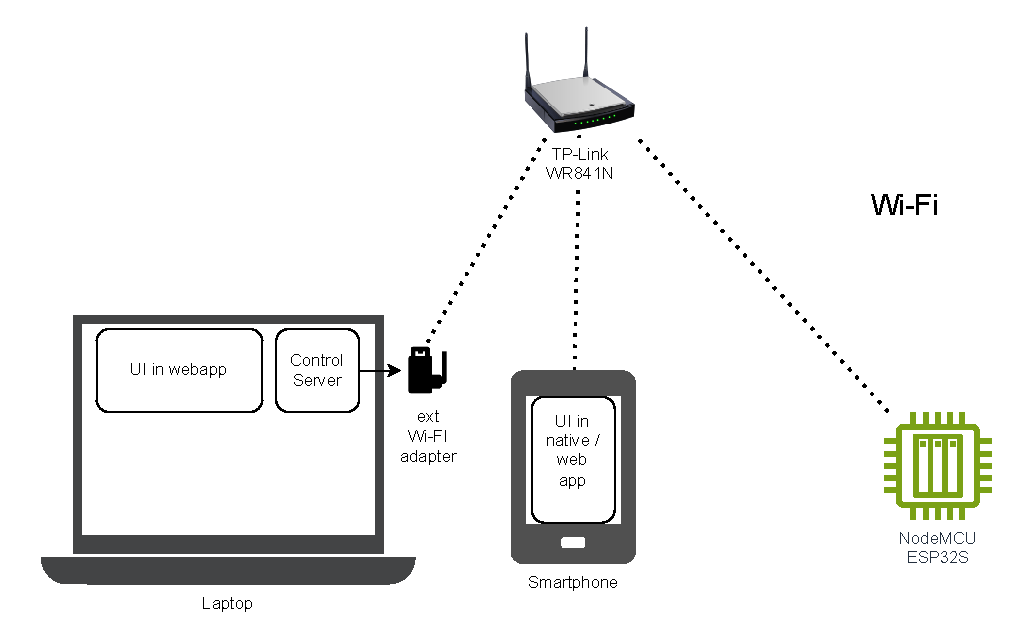
\includegraphics[page=1,keepaspectratio,width=150mm]{figures/box_network.drawio.pdf}
    \caption{Model network architecture}
    \label{fig:BoxNetwork}
\end{figure}

The communication medium between devices was chosen to be Wi-Fi, as this is one of the wireless protocols supported by microcontroller and by most laptops and smartphones, therefore a good common ground across devices. The control server was planned to be run on my own personal laptop for convenience and ease of development. Throughout Project Laboratory, I used a TP-Link WR841N at hand, which is a combined network device with routing, switching and Wi-Fi AP capabilities to symbolize a home network and provide a Wi-Fi network medium between devices. This remained in the the Thesis Project, with a custom firmware (DD-WRT) installed on it for more settings customization options, along with an extra Wi-Fi adapter plugged into the laptop for simultaneous usage of its internal Wi-Fi adapter to have Internet access. On \refstruc{fig:BoxNetwork}, a diagram of this network setup is shown.

One of the easily obtainable and connectable, yet spectacular electronic component that can be used in such a project is a Light Emitting Diode, or LED in short. A few LEDs and required resistors were obtained for the project in order to illuminate the rooms in a spectacular way, switched on or off from the user interface. Resistors of different common values were obtained to limit the current passing through components to protect them from overheating, for other devices as well, such as a light sensor in the form of an LDR (Light Dependent Resistor) and three LM235Z temperature sensors. For heating and cooling simulation, two 5V fans and a Peltier module were acquired. Two lower current rated BS170 and one BD241C transistors were obtained for powering the two fans and the Peltier module from a higher-current (2A) external 5V power supply (from a USB-charger). And finally, an SG90 servo was acquired and fitted with extra parts to simulate an automated electronic rolling shutter.

\section{Software environment}

At the end of Project Laboratory, the software architecture of the model box was comprised of three main components: a JavaScript backend responsible for maintaining the components' status and communication between the microcontroller and user, microcontroller code for controlling the electronic components (reading sensor data, setting output for actuators), receiving and sending data to the backend and finally a React-based frontend to send commands and receive readings to and from the backend. For the Thesis Project, I decided to replace it with already available open-source smart home system platforms with more functionalities and better device and community support, because I believe it would have been harder to further develop it in an extensible way, add more features and the integration itself was also a great technical challenge to be featured as a Thesis Project.

Choosing the right smart home software platform for the project is an essential task, because it is the foundation of the project and the other subsystems depend on it. Its features and offers, hardware and software support, community reception should be considered before fully commiting to it, because changing to a different one can be tedious work if it doesn't meet the set requirements. After researching the major open-source smart home software platforms on the Internet, two projects were considered: Home Assistant and OpenHAB. \cite{HAHomepage} \cite{openHABHomepage} Both projects have mostly the same to offer for a smart home platform: both are open-source, have good documentation, have built-in UI with customizations and integrations for many kinds of devices and options for automations. However, Home Assistant has a larger community of users, contributors and its popularity is also bigger (a Google Trends comparison also confirms this). \cite{WunderTechHAvsopenHAB} With these findings and recommendation from acquaintances in mind, Home Assistant was chosen to be the base smart home platform.

The microcontroller software platform is also important for the success of the project, it has to be compatible with the smart home platform, be stable and has to have support for required device types and automations. Platforms compatible with Home Assistant for the ESP32S architecture were searched for and two major projects were found: ESPHome and Tasmota. Both focus primarily on supporting ESP-based microcontrollers, have integration for Home Assistant, mostly have the same popularity and community support and have support for Over-the-Air (OTA) updates. \cite{ESPHomeHomepage} \cite{TasmotaHomepage} \cite{ESPHomeOTA} \cite{TasmotaOTA} The main difference between the two projects are the technologies used for transmitting messages between the control server and microcontroller: ESPHome mainly uses Event Source API, but also has support for a simpler REST API and Tasmota uses MQTT, a message queueing protocol. \cite{ESPHomeWebAPI} \cite{TasmotaMQTT} Both use JSON payloads for their messages, however the technologies used by ESPHome usually make the propagation of control and other messages faster than Tasmota. Eventually, the microcontroller software platform was chosen to be ESPHome.
% maybe esphome yaml files here, or in impl?

\chapter{Implementation}

The implementation of the box model, according to the plans discussed in the previous chapter, mostly went without issues and was able to be put into practice. This chapter presents the steps of implementation taken in detail.

\section{Floorplan}

\begin{figure}[!ht]
    \centering
    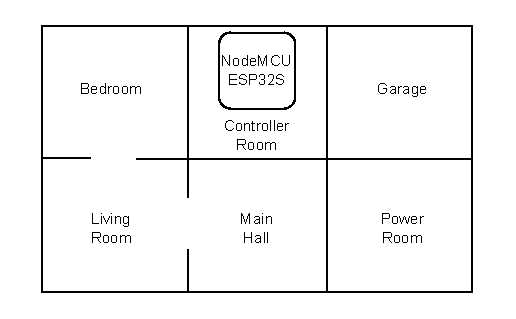
\includegraphics[page=1,keepaspectratio,width=110mm]{figures/box_floorplan.drawio.pdf}
    \caption{Floorplan of the finished box model}
    \label{fig:BoxFloorplan}
\end{figure}

The shoebox used as a base for the project was structured with cardboard and scotch tape to have six equal-sized rooms inside it, shown on \refstruc{fig:BoxFloorplan}. Internal and external cutouts were made in the box to be able to push cables through them, have ventilation holes for the fans, and have a window for the rolling shutter visible from outside.

\section{Connecting devices to the microcontroller}

\begin{figure}[!ht]
    \centering
    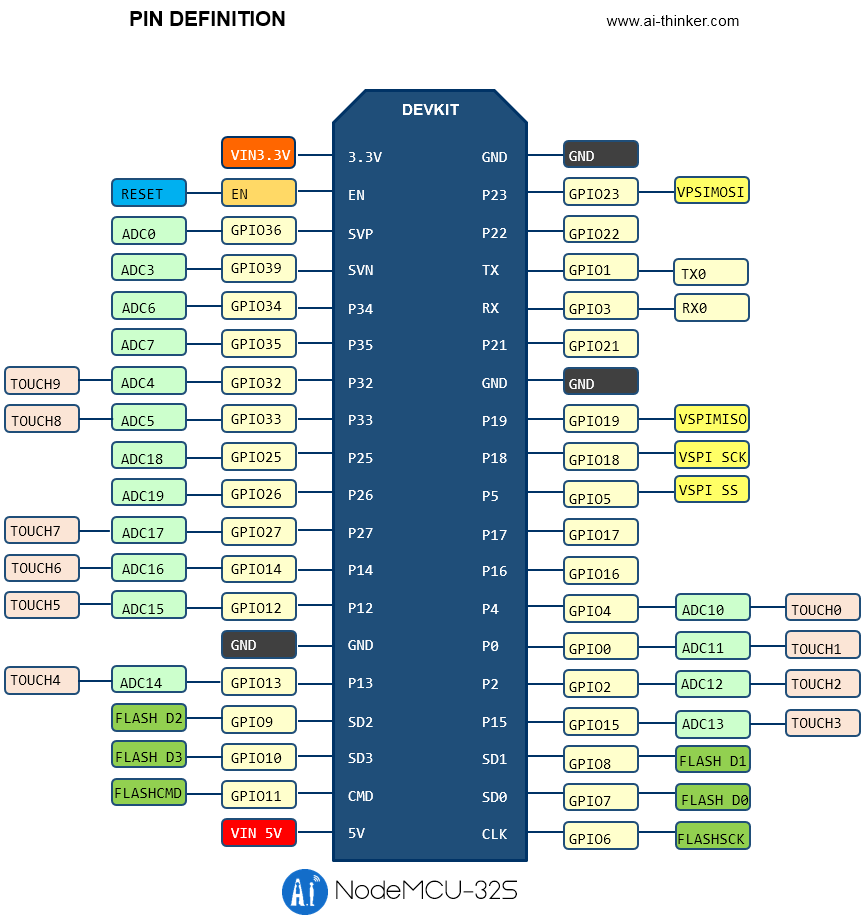
\includegraphics[width=150mm, keepaspectratio]{figures/nodemcu_32s_pinout.png}
    \caption{NodeMCU ESP32S Pinout}
    \label{fig:NodeMCU32Pinout}
\end{figure}

The NodeMCU ESP32S has many ports with different functionalities, as shown on \refstruc{fig:NodeMCU32Pinout}. \cite{AIThinkerNodeMCU32} It has a Micro-USB port that can be used for supplying power and connection to a computer for programming, flashing firmware and serial console. The 5V supplied from the USB port is connected to the VIN 5V pin and there is also a VIN 3.3V port from a voltage converter for supplying power to lower-voltage external components, besides the three ground (GND) pins. There are many more GPIO (General-Purpose Input/Output) pins with different input-output functionalities, however not every of them can be used for every purpose. For example, ADC/DAC pins can be used for Analog-Digital Conversion or vice-versa, therefore sense or create voltages between 0V and 3.3V, some can output PWM (Pulse Width Modulation) signals for dimming LEDs, controlling servos etc., serial pins can be used for serial communication, SD card interfacing and there are some only binary input-output pins. The 3.3V, 5V and ground pins were connected via short bendable solid cables to the power rail sides of the main breadboard for easy distribution of power to components. Jumper cables and wires were used to connect most components to the breadboards, which also served as extension to have appropriate length of cables for them and to be able to put into their desired location inside the box. The method for cable splicing varied, for some, soldering and shrink tubes were used and for others, only wire twisting and electrical tape was used due to the smoke detection system installed in the dormitory, where the project was mostly made.

\begin{figure}[!ht]
    \centering
    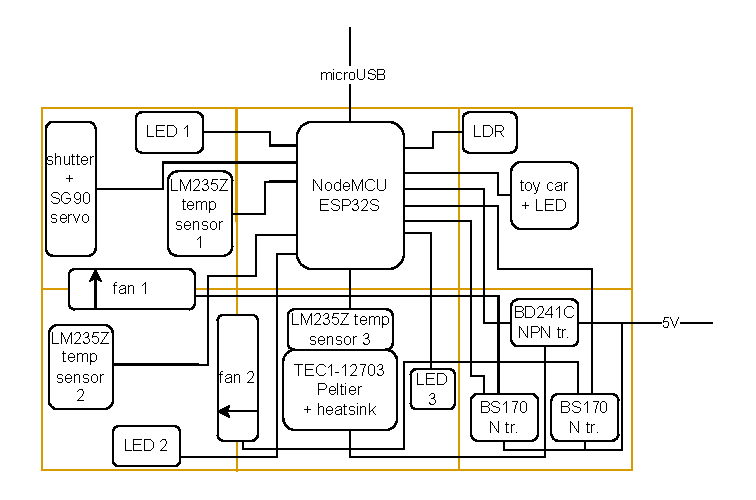
\includegraphics[page=1,keepaspectratio,width=150mm]{figures/box_block_diag.drawio.pdf}
    \caption{Simplified block diagram of components and their wirings inside the box}
    \label{fig:BoxBlockDiag}
\end{figure}

\begin{figure}[!ht]
    \centering
    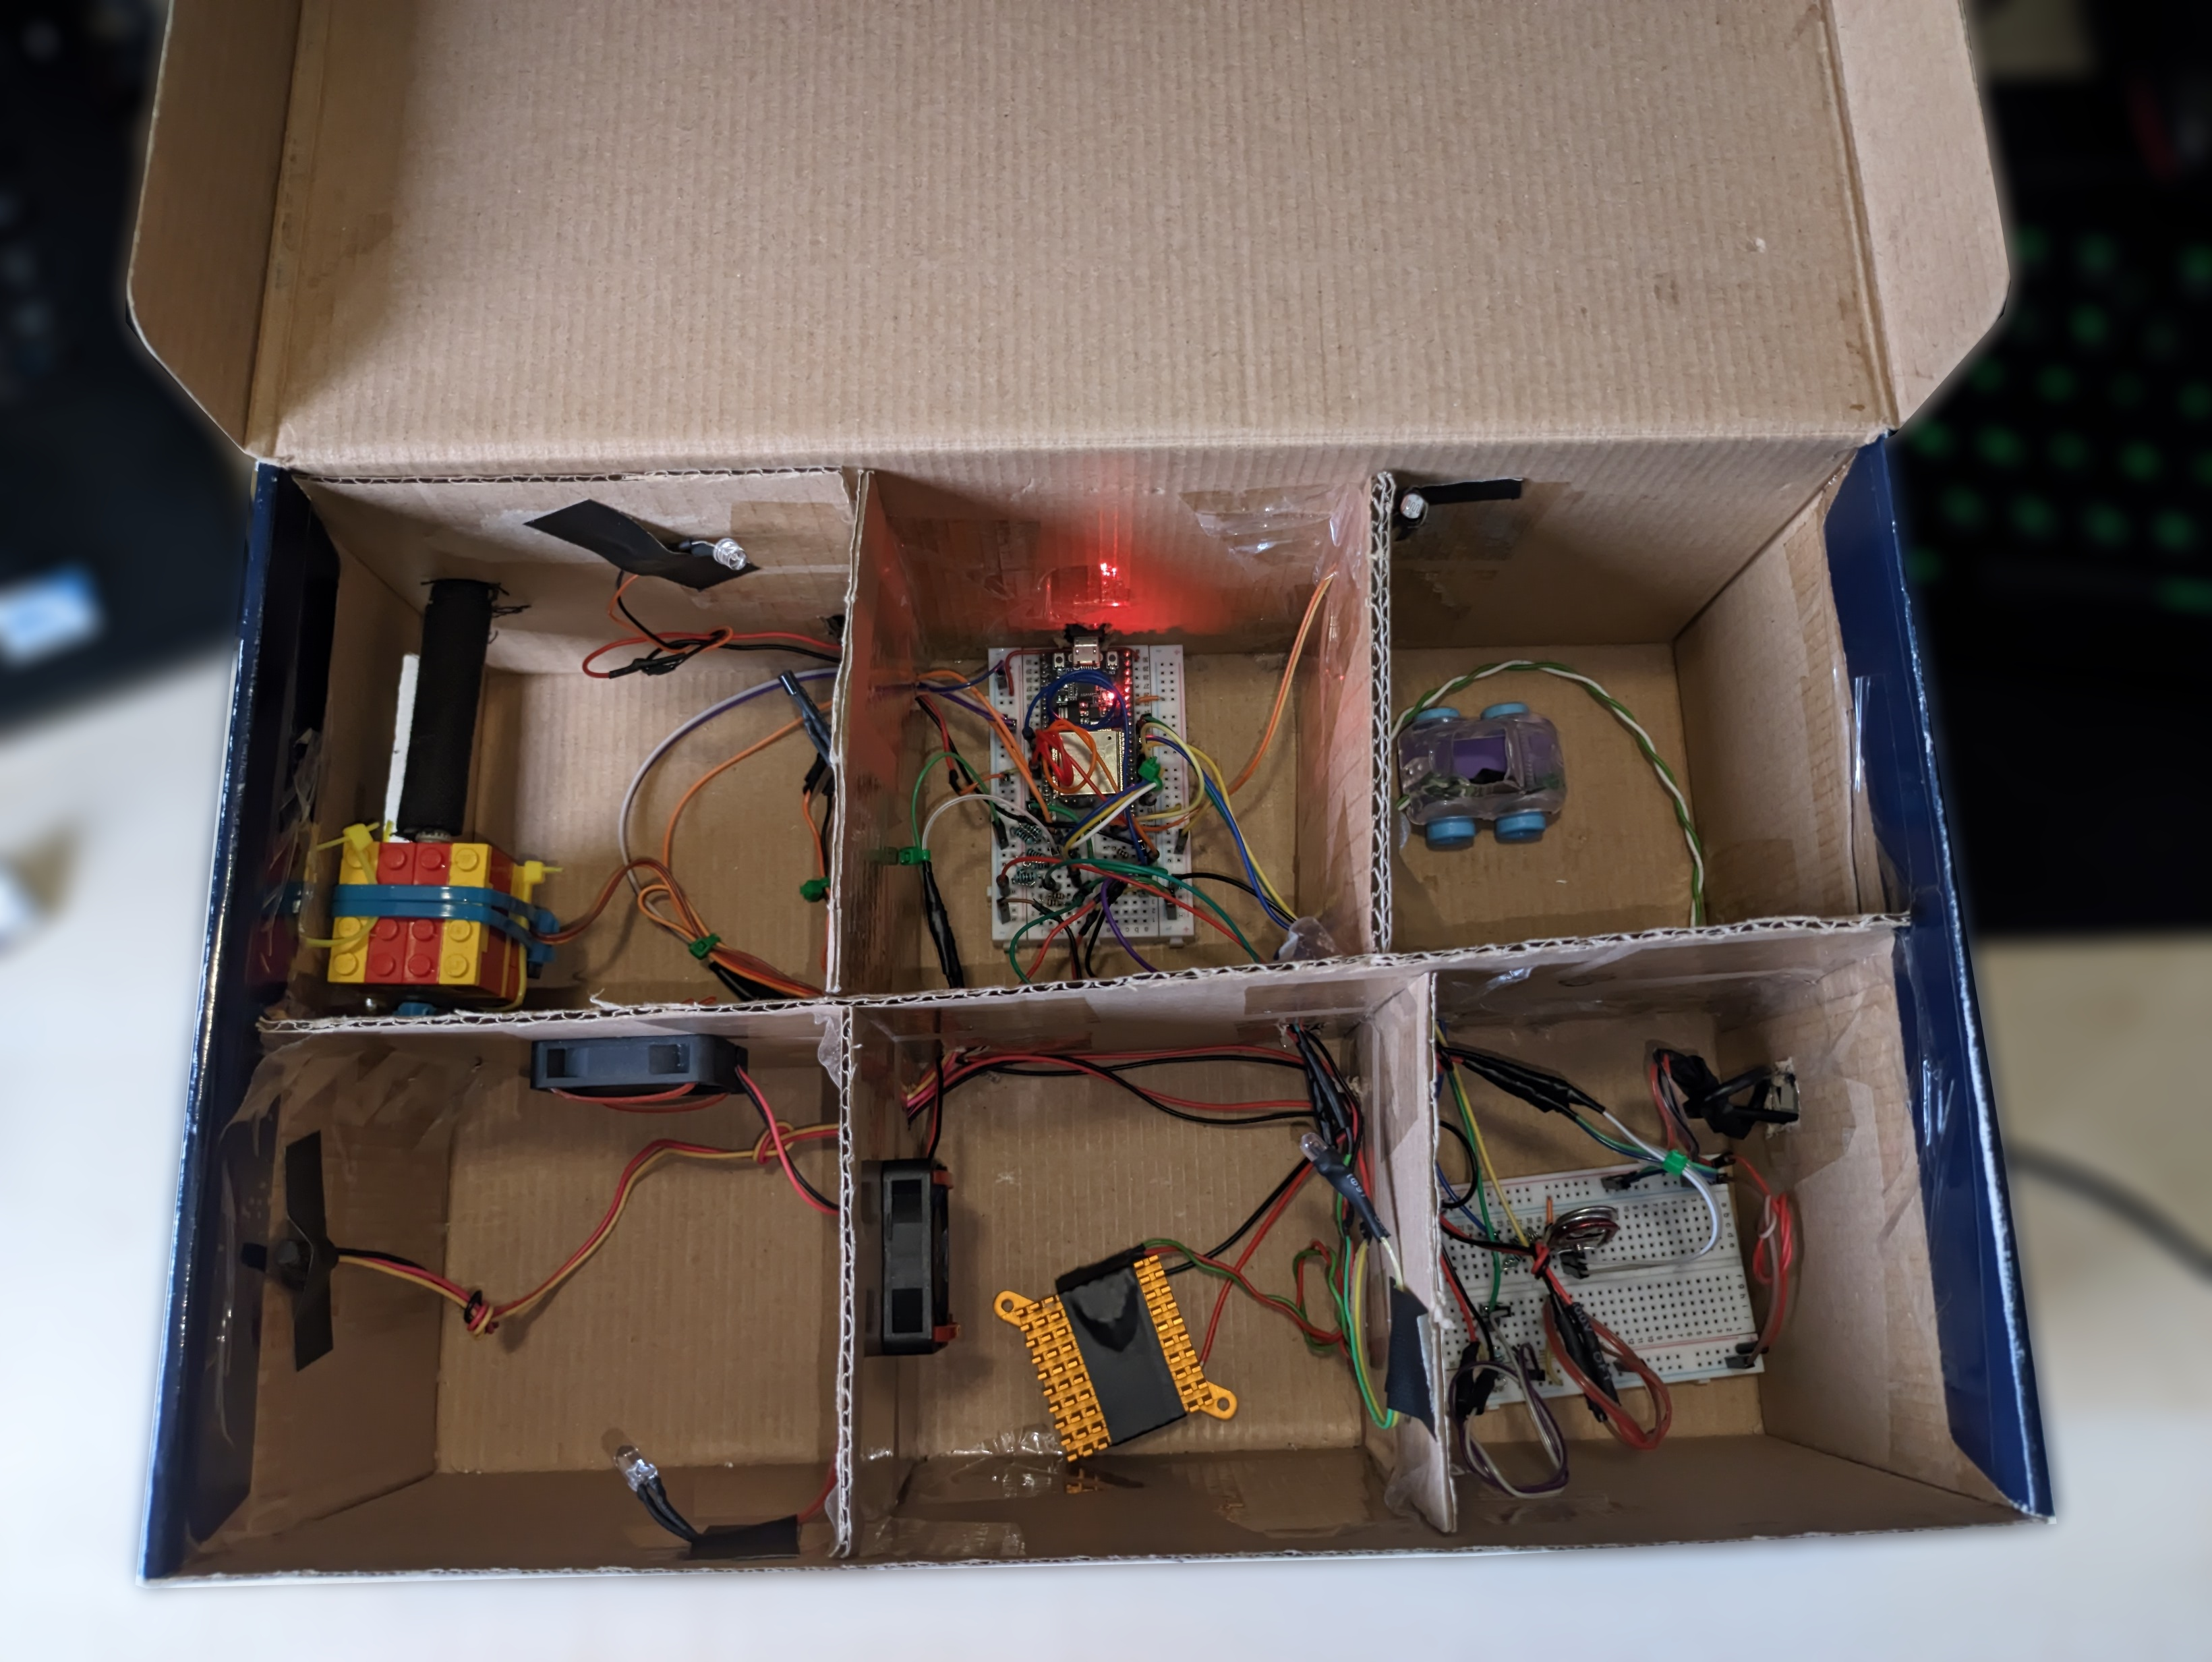
\includegraphics[width=150mm, keepaspectratio]{figures/box_photo.jpg}
    \caption{Photo of the finished box model}
    \label{fig:BoxPhoto}
\end{figure}

The microcontroller's number of pins and their functionalities were adequate the project, extra components can be added up to the limit the available free pins and the required features on them. The pins used for room LEDs were chosen to be non-ADC GPIO pins and for each one, 100$\Omega$ resistors were put between the LED's anode and the microcontroller pin, the cathode was connected to the side ground rail of the breadboard. An LED put inside a small toy car was also connected to a PWM-capable pin with 50$\Omega$ resistance in series to indicate a simulated electric car charging, based on the readings of the light dependent resistor (LDR). The LDR's wiring required a different approach: one end connected to the 3.3V rail, and the other to one of the microcontroller's ADC pins, and to the ground with a 10k$\Omega$ resistor. The three LM235Z temperature sensors were connected with yet another wiring method: 2k$\Omega$ resistors were put between 5V and their V+ terminals, to this the ADC pins were also connected and finally, the V- pins were connected to ground. The SG90 servo was connected to 5V, ground and a PWM capable pin for control. Due to the limited space remaining on the first breadboard, a second one was utilized for the fan and Peltier powering circuit. The ground between the two breadboards was connected with a jumper cable, and a USB cable with male jumper plugs spliced was created to utilize external power from a 5V 2A phone charger. The 5V fans are powered and speed controlled by BS170 transistors utilizing pulse width modulation (PWM). PWM-capable pins of the microcontroller were connected to the transistor's gate terminal, along with 10k$\Omega$ resistors to ground, the source terminal connected to ground and diodes placed between 5V and drain to protect the microcontroller from the inductive load of fans by only allowing flow of electricity in one way. The fans' negative terminals were connected to the transistors' drain and the positive to 5V. Finally, the TEC1-12703 Peltier module has a small heatsink taped onto it and is powered and controlled by a BD241C transistor (with extra cooling attached in the form of soda can tab openers screwed into it for more surface area). This Peltier module's maximum operating voltage is rated to be 15.4V, which means, when run at a lower voltage, it draws less current, therefore functions with a lower power. According to its datasheet, at 5V (which is given by the USB charger), its current is approximately 0.8A, therefore the device draws about 4 watts of power and it decreases with more ambient temperature as the current gets less. \cite{PeltierDatasheet} 333$\Omega$ resistance was used between one of the DAC pins and the transistor's base, the emittor was connected to ground and the Peltier's terminals were connected to the collector and 5V. In \refstruc{fig:BoxBlockDiag}, a simplified block diagram of components and their wirings inside the box is shown without resistors, ground connections, exact pinout of components, and on \refstruc{fig:BoxPhoto}, a photo of the finished box model is shown with the microcontroller turned on.

\section{Network setup}

The Wi-Fi communication medium was set up using a TP-Link WR841N combined network device, targeted for small or home office use. Such devices almost always feature a web-based user interface for their setup and configuration. This was used to flash DD-WRT on it, which is an open-source Linux-based router firmware targeting a variety of Wi-Fi routers and embedded systems. \cite{DDWRTHomepage} It was then set up to mimick a typical home environment, with an SSID of esp\_smart\_home, WPA2-PSK authentication, without internet connectivity and without NAT (Network Address Translation, by setting the operation mode from gateway to router). The IP address range remained the default 192.168.1.0/24 and the router's IP also remained the initial 192.168.1.1, due to it not colliding with other networks actively used on the laptop and smartphone.

An extra Realtek chip based USB Wi-Fi adapter at hand was used for connecting the laptop to the Wi-Fi network, with a custom network profile configuration. Initially, the use of this adapter was done with a network profile limited to the specific network adapter and manual IP configuration was used instead of DHCP to ensure a fixed IP address of 192.168.1.100 and no default gateway learned from this network. Later, it was passed through as a USB device to a virtual machine (VM) with the same Wi-Fi and IP configuration. The Android-based smartphone used for the project was also connected to this network, but didn't have internet connection despite having an Internet-capable SIM card put into it meant as a fallback connection, according to the gained experience.

\section{Software setup}

The chosen software environment discussed in the planning phase was suitable for the usage of obtained hardware, this section showcases the steps taken for its software setup. The personal laptop used for development had a Linux distribution installed, the smartphone used for testing ran Android 14.

\subsection{HomeAssistant initial setup, migration}

Initially, Home Assistant was set up in a Docker container environment running on the laptop, with a Docker Compose file specifying the parameters for the container. Docker Engine is a container runtime engine, that makes it possible to run prepackaged container images utilizing the host machine's kernel with minimal overhead and adequate isolation. \cite{DockerContainer} The container images contain a Linux operating system's system libraries, executables and the application itself, therefore provide an easily reproducible, uniform runtime environment despite the differences in various systems. By itself, Docker has a command line interface to run and manage its containers, which means it has to be parameterized from the command line, or put into a script in its parameterized form and executed. Docker Compose is a solution for defining and running multiple Docker containers using an easy-to-manage definition, put into a YAML file. \cite{DockerCompose} YAML is a human-friendly data serialization language with a really simple syntax, as shown in \refstruc{lst:YAMLexample}. \cite{YAMLHomepage}

\begin{lstlisting}[language=,caption=YAML file example,label=lst:YAMLexample]
  shopping_list:
    - bread
    - milk
    - chocolate

  # ideal room temperature
  temperature: 22

  winter_months: ["December", "January", "February"]
\end{lstlisting}

In \refstruc{lst:HADockerCompose}, the Docker Compose definition of the set up Home Assistant container can be seen: 2024.10.3 is the selected version (tag) of the image is used, the config directory from the compose file's directory is mounted directly into the container's file system as /config along with the host machine's local time and dbus for time and device access, and finally, socket connections are bound on the host machine's 8123 port on the Wi-Fi card and localhost interfaces to access the same port inside the container.\break

\begin{lstlisting}[language=,caption=Docker Compose file used for the initial Home Assistant environment,label=lst:HADockerCompose]
services:
  homeassistant:
    container_name: homeassistant
    image: "ghcr.io/home-assistant/home-assistant:2024.10.3"
    volumes:
      - ./config:/config
      - /etc/localtime:/etc/localtime:ro
      - /run/dbus:/run/dbus:ro
    ports:
      - 192.168.1.100:8123:8123
      - 127.0.0.1:8123:8123
\end{lstlisting}

Even though only one container is defined in the compose file, it still shows Compose's advantage, as the environment can be run with a simple command in the terminal, when inside the compose file's directory:

\begin{lstlisting}[language=]
docker compose up
\end{lstlisting}

This setup in the Docker environment functioned properly, however had one limitation: HomeAssistant add-ons aren't supported in the container variant, only in the Home Assistant Operating System (HA OS) or the Supervised installation (installed on top of a Linux installation) variants. A voice assistant was a sought after feature in the project, therefore it was migrated to the HA OS variant, run inside a virtual machine, or VM.

Virtual machine hypervisors allow physical, or host computer resources to be shared to multiple virtual machines, or guest machines. \cite{VMwareVM} Each virtual machine can run it's own separately with its own amount of CPU cores, RAM, storage and other kinds of resources. Virtual Machines are widely used today in IT infrastructures, as the technology makes it easier to create heterogeneous software environments and can offer less downtime with clusterized servers. The most popular current virtualization solutions include VMware products, Oracle VirtualBox and Proxmox. \cite{G2freeVM}

\begin{figure}[!ht]
  \centering
  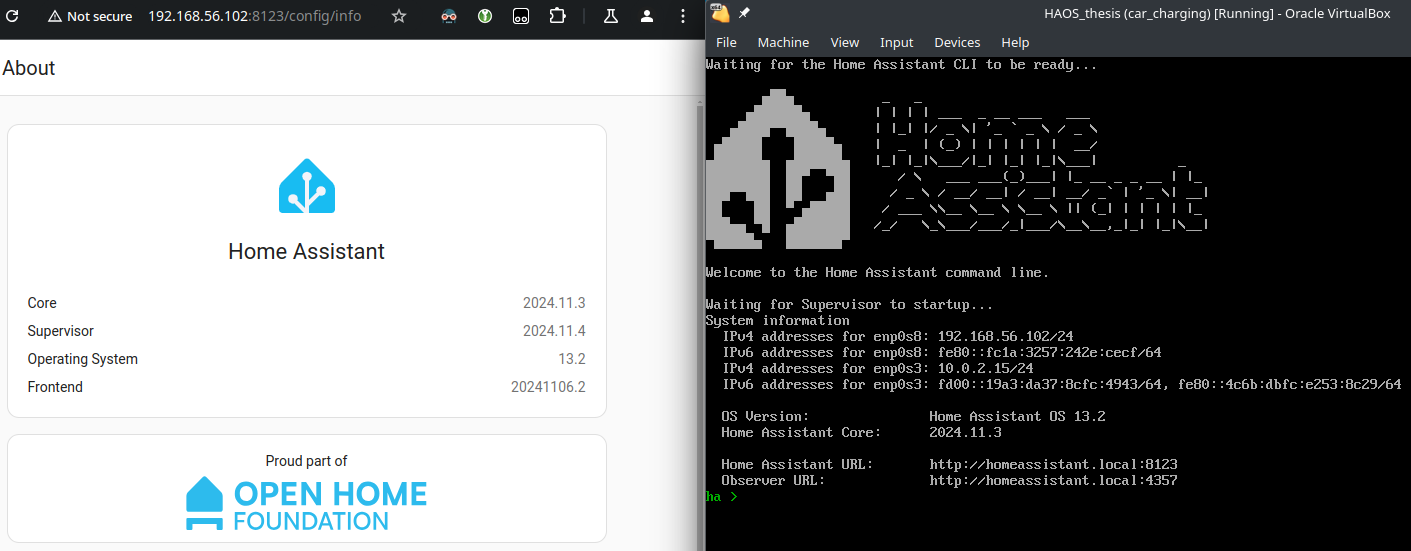
\includegraphics[width=150mm, keepaspectratio]{figures/homeassistant_about.png}
  \caption{Home Assistant OS running in VirtualBox with its web GUI opened from a browser}
  \label{fig:HAabout}
\end{figure}

To run HA OS, the selected VM hypervisor solution was Oracle VirtualBox, due to it being free and and the previous experience gained with it in the past. HA OS is distributed in different disk file formats for various hypervisors, VDI was used for VirtualBox.
Initially, 2 virtual CPU cores and 2 GB of RAM of the host's 16 GB was assigned to it, however it was later changed to 4 GB of RAM to run the voice assistant functionality faster. Two virtual network adapters were added to the VM: one in NAT mode, to provide Internet connection for updates and downloading add-ons, and one adapter in Host-only adapter mode, to be able to be reached from the host (on it's web UI (8123) and SSH (22) ports). Most VM hypervisors offer USB passthrough to virtual machines, which hides the USB device from the host and makes it seem as it was connected to the VM directly. USB passthrough was used to access the USB Wi-Fi adapter inside the VM and the network credentials were set via a parameterized \verb+ha network+ command with the specific SSID, password and IP configuration. The SSH addon was also installed to access command line configurations from a client terminal installed on the host operating system. The configuration of the new environment (eg. integration and dashboard setups) didn't needed to be redone from scratch, as the old environment could be exported to a tar backup file, which was then able to be imported to the new HA OS environment without issues during its initial setup from the web GUI.

\subsection{ESPHome}

To get started with installing ESPHome on the microcontroller, its official getting started with command line guide was followed. \cite{ESPHomeGettingStarted} A sample configuration YAML file was created using the wizard command. The ESPHome compiler and flasher was run from a Docker environment, first flashed via USB and later updated wirelessly using ESPHome's the Over-the-Air (OTA) functionality via Wi-Fi.

\begin{lstlisting}[language=,caption=Docker command to compile and flash ESPHome via OTA / USB,label=lst:ESPHomeDocker]
# for first flashing, add: --device=/dev/ttyUSB0
docker run --rm -v "./esphome":/config -it ghcr.io/esphome/esphome:2024.11.1 run smarthome.yaml
\end{lstlisting}

By default, an ESPHome configuration file only consists of one main YAML file, which contains all configurations. On \refstruc{lst:ESPHomeWizardEx}, an excerpt of a configuration file is shown generated by the wizard for the NodeMCU ESP32S microcontroller.

\begin{lstlisting}[language=,caption=Excerpt of a configuration file generated by the ESPHome wizard,label=lst:ESPHomeWizardEx]
esphome:
  name: livingroom
esp32:
  board: nodemcu-32s
  framework:
    type: arduino
ota:
  - platform: esphome
    password: ""
wifi:
  ssid: "homenetwork"
  password: "teriyaki-noodles"
\end{lstlisting}

\begin{figure}[!ht]
  \centering
  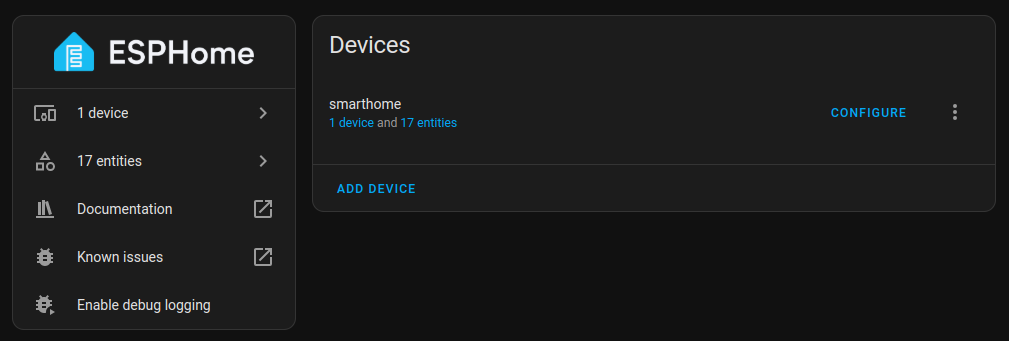
\includegraphics[width=150mm, keepaspectratio]{figures/homeassistant_esphome_int.png}
  \caption{ESPHome integration for Home Assistant set up}
  \label{fig:HAesphomeint}
\end{figure}

After successfully flashing the compiled firmware to the microcontroller, it can then be added to the Home Assistant environment with an "integration". Integration is a term in Home Assistant's ecosystem to connect and integrate other software and hardware platforms, in our case ESPHome to the Home Assistant environment as a device. \cite{HAConceptsTerminology}

ESPHome supports many types of electronic components connected to the microcontroller's pins (as the project's homepage shows), with a relatively easy configuration. \cite{ESPHomeHomepage} To set devices up to be utilized by ESPHome, their configuration has to be defined in the YAML configuration file, as shown in \refstruc{lst:ESPHomeDevConf} for a switch, that toggles an LED. Each device should have an \verb+id+ and \verb+name+ set, along with platform specific details, such as the GPIO pin number and mode (input / output).

\begin{lstlisting}[language=,caption=ESPHome configuration for a simple LED switch,label=lst:ESPHomeDevConf]
switch:
- platform: gpio
  id: bedroom_led
  pin:
    number: GPIO21
    mode: OUTPUT
  name: "BedroomLED"
  restore_mode: ALWAYS_OFF
\end{lstlisting}

This configuration was also done iteratively to the other connected components as well, but in separate files with the use of packages, which is a functionality provided by ESPHome for better code structuring and maintainability. With packages, ESPHome configurations are merged from multiple YAML files to a single one during compilation, as if they were written in that single one.

\begin{lstlisting}[language=,caption=ESPHome package includes in the main configuration file,label=lst:ESPHomePackageIncludes]
packages:
  fans: !include packages/fans.yaml
  ldr: !include packages/ldr.yaml
  leds: !include packages/leds.yaml
  peltier: !include packages/peltier.yaml
  shutter: !include packages/shutter.yaml
  tempsensors: !include packages/tempsensors.yaml
\end{lstlisting}

\begin{figure}[!ht]
  \centering
  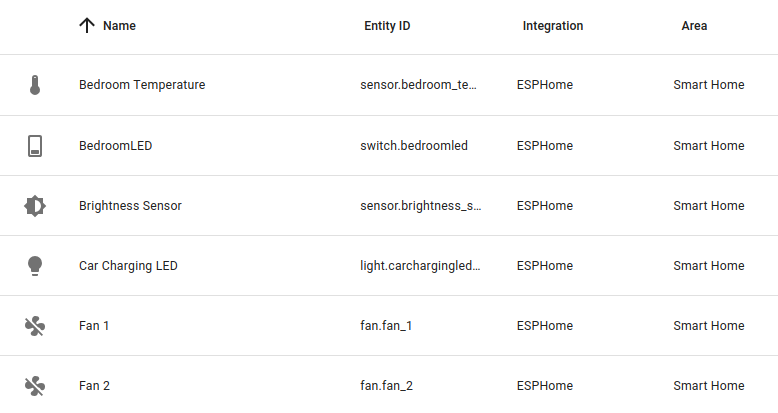
\includegraphics[width=150mm, keepaspectratio]{figures/esphome_entities.png}
  \caption{Home Assistant entities provided by the ESPHome integration}
  \label{fig:HAesphomeEntities}
\end{figure}

After reconfiguring the microcontroller with extra devices, Home Assistant automatically takes care of the devices added and new entities are created for them. In Home Assistant's terminology, entities are the basic building blocks that hold data and are used to monitor physical properties or control entities. \cite{HAConceptsTerminology} On \refstruc{fig:HAesphomeEntities}, a few entities from the ESPHome integration device are shown. 

\begin{figure}[!ht]
  \centering
  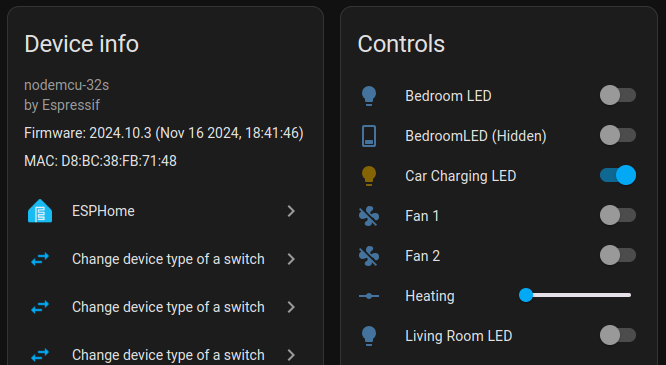
\includegraphics[width=150mm, keepaspectratio]{figures/esphome_controls.png}
  \caption{Device of the ESPHome integration and its control entities}
  \label{fig:HAesphomeControls}
\end{figure}

The ESPHome integration's device, its controls, sensors and configurations can also be seen and configured, as shown on \refstruc{fig:HAesphomeControls}.

One component connected to the microcontroller was harder to be configured for use, than others, which is the SG90 servo used for the rolling shutter. Fortunately, other ESPHome users had also tried to make this exact servo model work and one forum member was able to and provided configuration code for it, which includes PWM configuration, conversion of value from a number slider's -100 to 100 range to the servos 180 degrees of control and a sensor for the currently set position. \cite{ESPHomeForumSG90} This example superbly shows an advantage of open-source software and its communities, how projects can be easily extended with extra, more complex components and how users can get support for their problems.

\subsection{Additional user interface setup, customization}

\subsubsection{Entity customization}

\begin{figure}[!ht]
  \centering
  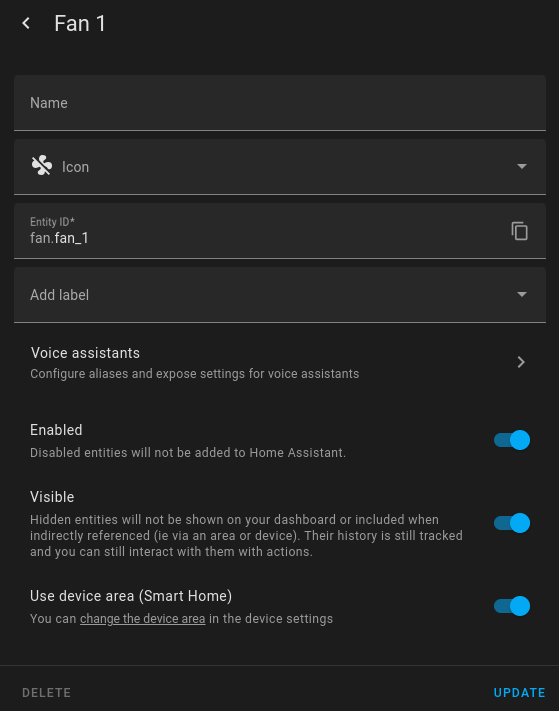
\includegraphics[width=90mm, keepaspectratio]{figures/homeassistant_entity_customization.png}
  \caption{Entity customization in Home Assistant}
  \label{fig:HAentityCustomization}
\end{figure}

Customizations can be applied on Home Assistant entities to better suit the user's needs. Each entity has a unique id, which is used as a basis to uniquely identify a specific entity and it is guaranteed to be static and never changes. \cite{HAFAQUniqueID} When present, it gets assigned an entity id, which is in the form of \verb+<domain>.<id>+ and is used as a logical identifier in dashboards, automations and others. \cite{HAEntitiesDomains} To give examples, \verb+fan.fan_1+ is in the \verb+fan+ domain, therefore can be controlled as a fan, has an id of \verb+fan_1+ and \verb+light.bedroom_led+ is a light with an id of \verb+bedroom_led+. The entity id can be changed if desired, but it has to be unique throughout the Home Assistant environment. And finally, each entity has a \verb+name+, which is used as a display name and is displayed on dashboards, can be referrered to in the voice assistant, etc. Besides a name and id, an icon and labels can also be specified, as shown on \refstruc{fig:HAentityCustomization}.

\begin{figure}[!ht]
  \centering
  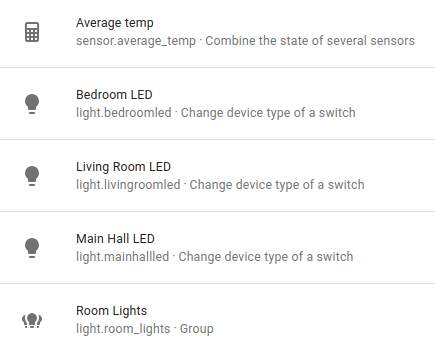
\includegraphics[width=110mm, keepaspectratio]{figures/homeassistant_helpers.png}
  \caption{Home Assistant helpers used in the project}
  \label{fig:HAhelpers}
\end{figure}

Helpers are software tools to add or change functionality of different entities. For example, the states of multiple devices can be combined to a single value (eg. to calculate the average temperature in the house), change the type of a switch to a different device (eg. togglable binary light, fan, lock) or combine multiple entities into a single virtual entity with the usage of the group feature. On \refstruc{fig:HAhelpers}, the helpers used in the project are shown.

\subsubsection{Dashboard customization}

Multiple dashboards can be created in Home Assistant to control and show different aspects and devices of a house. Upon setup, a default dashboard is automatically created, the layout of which is shown on \refstruc{fig:HAdefaultDashboard}.

\begin{figure}[!ht]
  \centering
  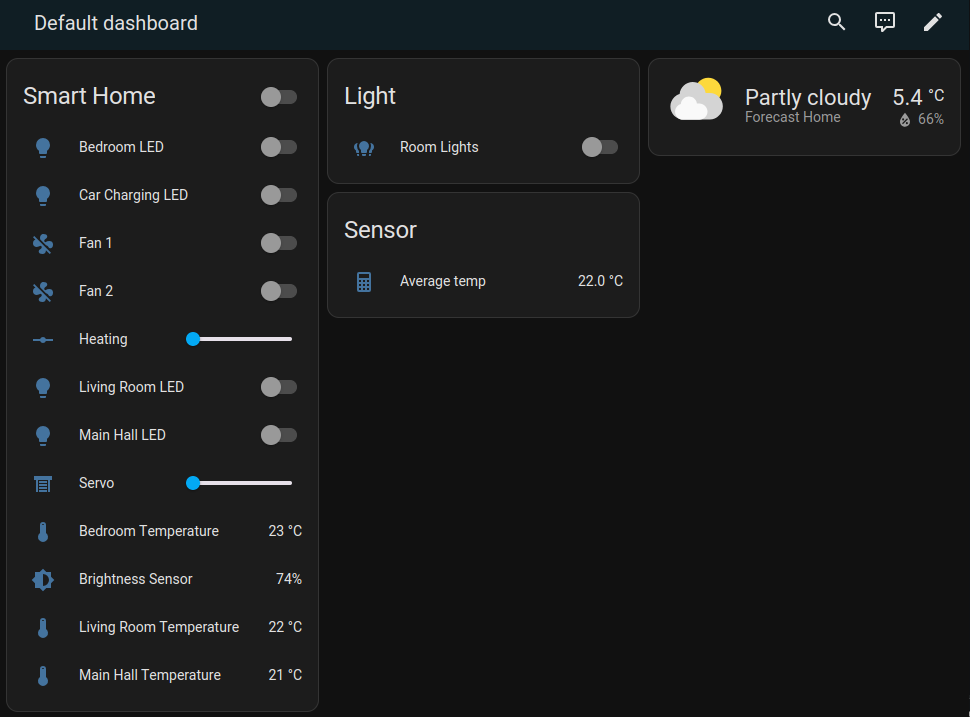
\includegraphics[width=150mm, keepaspectratio]{figures/homeassistant_dashboard_default.png}
  \caption{Default dashboard layout with controls and readings for the box device and weather forecast integration set to Budapest}
  \label{fig:HAdefaultDashboard}
\end{figure}

\begin{figure}[!ht]
  \centering
  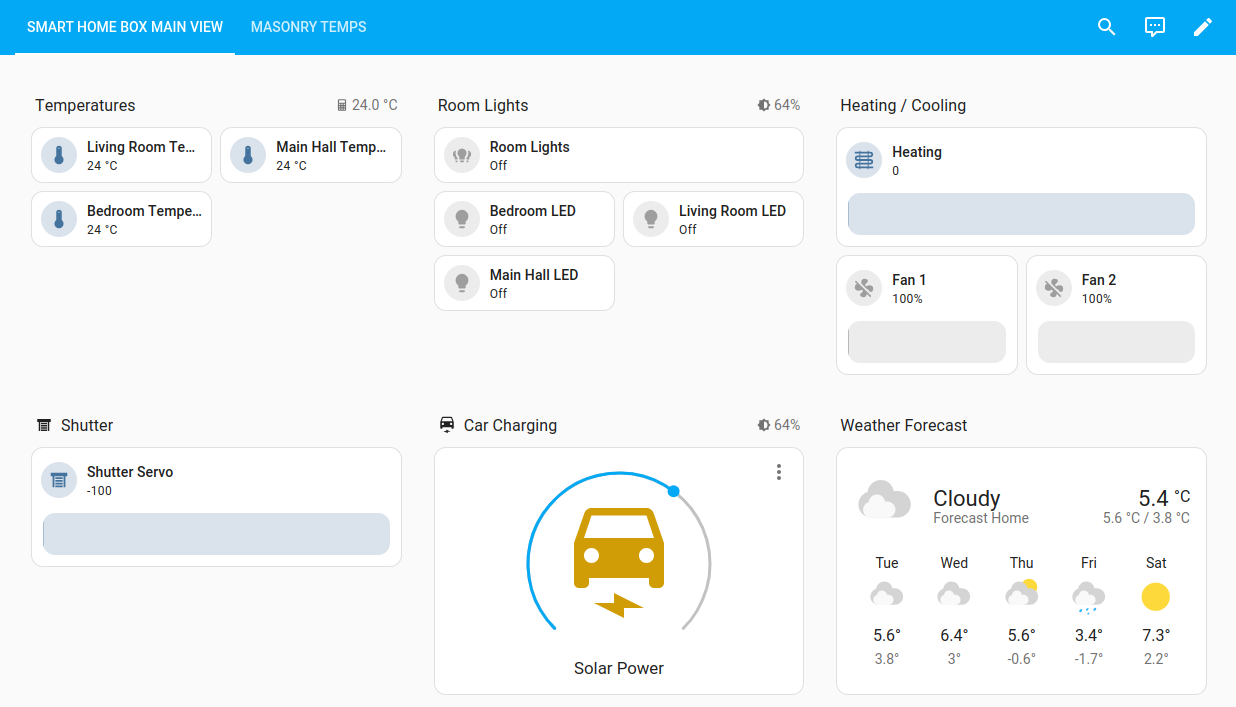
\includegraphics[width=150mm, keepaspectratio]{figures/homeassistant_dashboard_custom.png}
  \caption{Custom sections dashboard with devices grouped together by type and weather forecast integration set to Budapest}
  \label{fig:HAcustomDashboard}
\end{figure}

\begin{figure}[!ht]
  \centering
  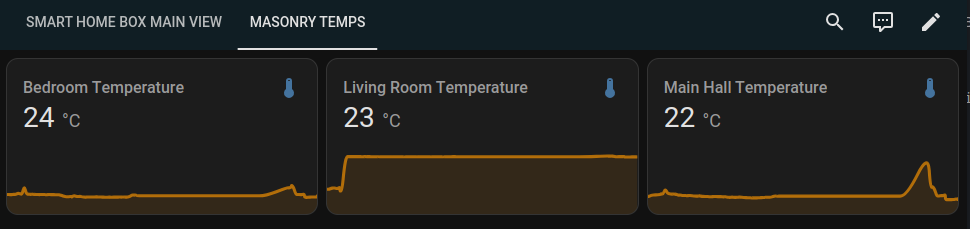
\includegraphics[width=150mm, keepaspectratio]{figures/homeassistant_dashboard_masonry.png}
  \caption{Masonry dashboard layout with historical graphs for room temperatures}
  \label{fig:HAmasonryDashboard}
\end{figure}

On the default dashboard, all areas, device controls and readings, integrations are shown as a whole, which can be ideal for a typical home environment with multiple devices, but not for the project with basically a single device and its many entities. Therefore another dashboard with a sections type view was created, which is shown on \refstruc{fig:HAcustomDashboard}. Multiple sections were created for the various types of controls (eg. lights, fans) and sensors (room temperatures), which were grouped together by the types of entities. Additional extra entities were added three sections for display: the average temperature of the three rooms to the "Temperatures" section and the LDR sensor's value to the "Room Lights" and "Car Charging" sections. The car charging section mimicks electric car charging with imaginary solar panels (actually based on the value of the LDR): the set brightness of the automated LED is used as the value for display, click events on the section were disabled to make it read-only (from this dashboard).
% maybe areas, labels, zones(osm)?

A masonry type view was also added to the dashboard, which is shown on \refstruc{fig:HAmasonryDashboard}. When multiple views are present for a dashboard, a tab strip is shown to select between them, as shown on the screenshot. On the masonry view, added cards are sorted in columns based on their sizes, three equal sized historical graphs were added of the room temperatures recorded.

\subsection{Smartphone setup}

Besides having a web-based UI, Home Assistant also has mobile applications for the Android and iOS platforms called Home Assistant Companion. \cite{HACompanion} To test the mobile application, it was installed to a personal Android smartphone. The smartphone was connected to the Wi-Fi network with its credentials, and the IP address of the HA OS VM Wi-Fi adapter with the proper protocol and port (\verb+http://192.168.1.100:8123+) was entered into the application as the instance URL. On \refstruc{fig:HAandroidScreenshot}, a screenshot of the Android application is shown.

\begin{figure}[!ht]
  \centering
  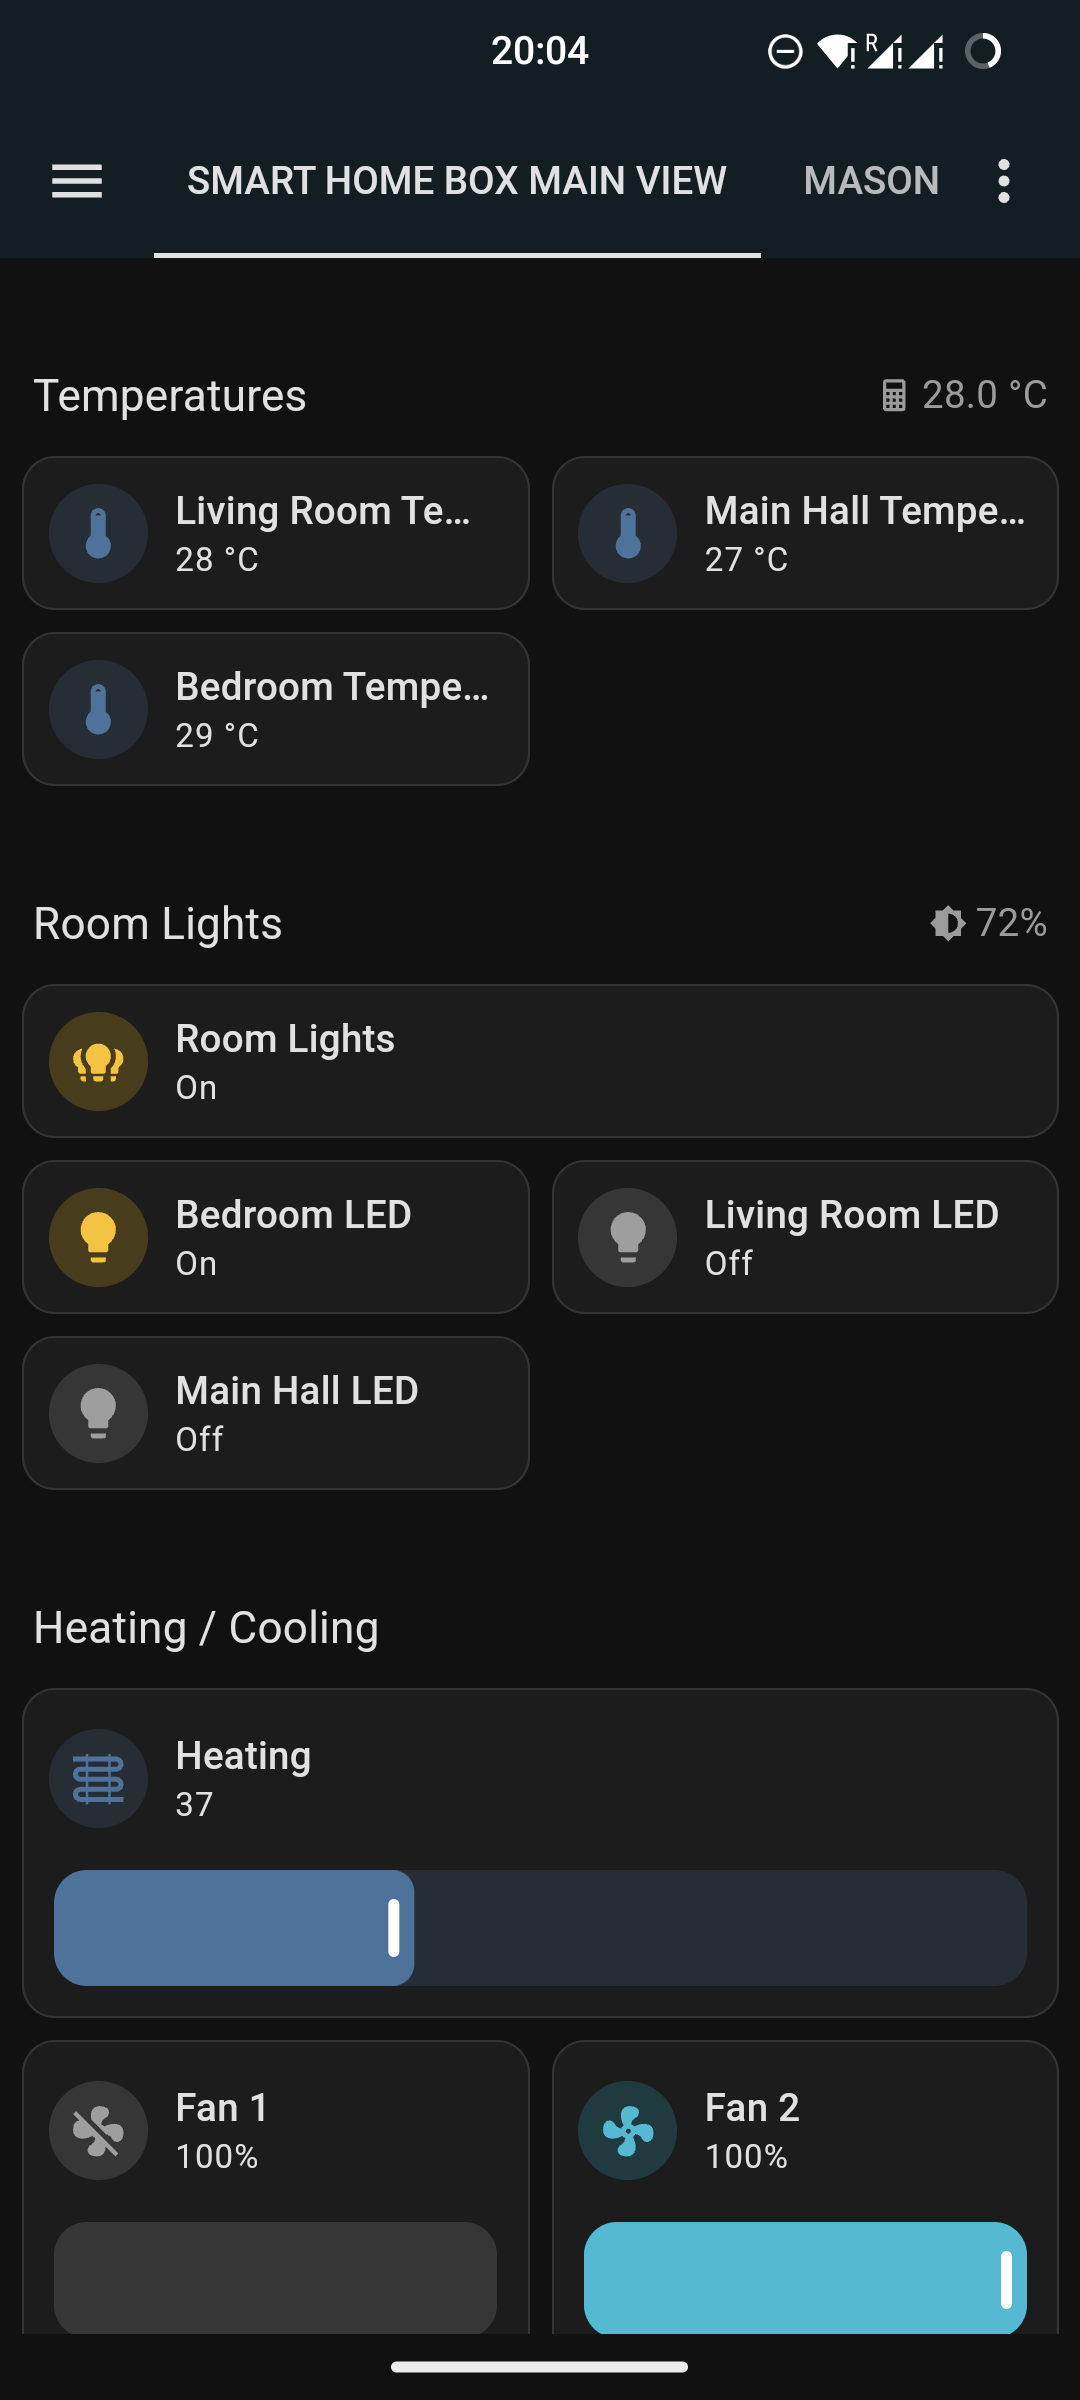
\includegraphics[width=70mm, keepaspectratio]{figures/homeassistant_android_screenshot.png}
  \caption{Home Assistant Companion app running on Android 14}
  \label{fig:HAandroidScreenshot}
\end{figure}

Contrary to expectations, simultaneous use of the the Internet-less Wi-Fi network and the phone's data-enabled SIM card for Internet connection didn't work, even if the "Mobile data always active" option was turned on in the developer settings. A message is shown when connecting to the network about it not having an Internet connection and whether the phone should stay connected to it and only upon pressing yes, can the server be reached. But at the same time, the status bar shows that LTE disappears, which can mean that the radio data connection is dropped or only the routing table is changed, but in such a way that the default gateway gets overriden to the Wi-Fi network. It would likely be possible to be able to change this behaviour with a rooted phone (where a root shell access is present), but its risks and disadvantages aren't worth it for this simple test scenario. And in a typical home network environment, where there wouldn't be a need to access two networks simultaneously, the HA OS server and the Internet would be able to be reached at the same time.

\subsection{Automations}

To make the life of its users easier and more comfortable, Home Assistant offers automations to run specific tasks. An automation comprises of three parts: triggers (when it runs), conditions (optional, only run if these conditions are met) and actions (what actions to perform). \cite{HAAutomationBasics} Besides basic automations, there are further features closely related to them: scenes can be used to set a group of entities to a specified state, scripts can contain multiple actions and blueprints can be used to specify a generic automation framework, which can be used as a common basis for multiple different automations with exactly specified entities.

During Project Laboratory, one feature that the model box had is the ability to show "solar power" by changing the brightness of the LED put inside a toy car based on the readings of the LDR. This was possible to replicate in Home Assistant too, with the use of an automation. Two kinds of triggers were tried for detecting when the automation should run: the first was using "Brightness Sensor voltage change", however even with a very small duration specified (1-5 seconds) between 0 \% and 100\% set as the voltage percent range, the automation wasn't triggered frequently enough, only about once a minute. Therefore an other trigger was used: a periodic interval of 5 seconds, which works reliably and its configuration is shown on \refstruc{fig:HAautomationTrigger}.

\begin{figure}[!ht]
  \centering
  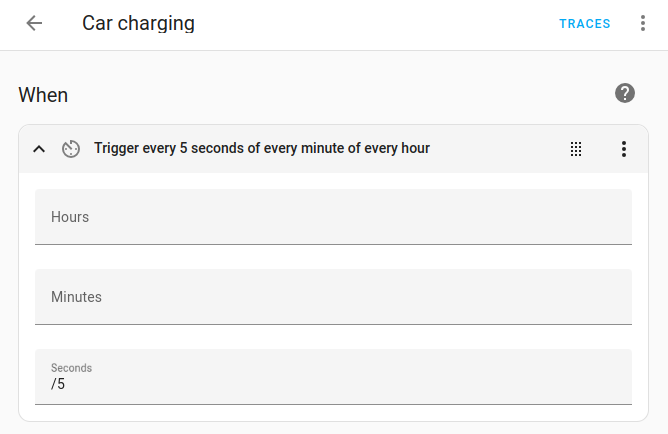
\includegraphics[width=110mm, keepaspectratio]{figures/homeassistant_automation_trigger.png}
  \caption{Home Assistant automation trigger}
  \label{fig:HAautomationTrigger}
\end{figure}

The action needed to accomplish one simple task: set the brightness value of the car charging LED, based on the readings of the LDR. This was possible to be defined via the YAML editor (the set content is shown in \refstruc{lst:HAautomationAction}), as the visual editor would have only allowed a constant number to be set as brightness. For action, \verb+light.turn_on+ was specified, that turns on the specified target light entity (which is \verb+light.car_carging_led+, if it isn't on already) and a \verb+brightness_pct+ data key is also specified, which tells \verb+light.turn_on+ what the target light's brightness should be set to. This key is defined to be the result of a template (inside double curly braces): \verb+states()+ retrieves the value of the LDR reading, which is in the form of an integer between 0 and 100 and it gets set to be \verb+brightness_pct+.

\begin{lstlisting}[language=,caption=Home Assistant automation action for setting LED brightness based on LDR,label=lst:HAautomationAction]
action: light.turn_on
metadata: {}
data:
  brightness_pct: "{{ states('sensor.brightness_sensor') }}"
target:
  entity_id: light.car_carging_led  
\end{lstlisting}
\break

\subsection{Voice assistant}

As a prerequisite for the locally hosted voice assistant, the Home Assistant Docker environment was migrated to HA OS running in a VM, explained with more details in chapter 3.4.1. To set up the voice assistant environment, the installation guide was followed to set up the Piper (text-to-speech) and Whisper (speech-to-text) add-ons. \cite{HALocalAssist} The add-ons were configured to use a low quality speech detection and synthetization, in order to ensure fast response, as even with medium, the response time dramatically increased after pronouncing the commands. A screenshot of the assistant can be seen on \refstruc{fig:HAandroidVoiceAssistant}. The speech detection and synthetization supports many languages to be configured: English (UK, US), German and Hungarian were tried and out of these, English had the best accuracy of understanding and executing the said commands. Although it is impressive, it only works with simple commands, when exact device names are specified and doesn't reach the level of Artificial Intelligence based chatbots, that gained a rapid technology boom in the last few years.

\begin{figure}[!ht]
  \centering
  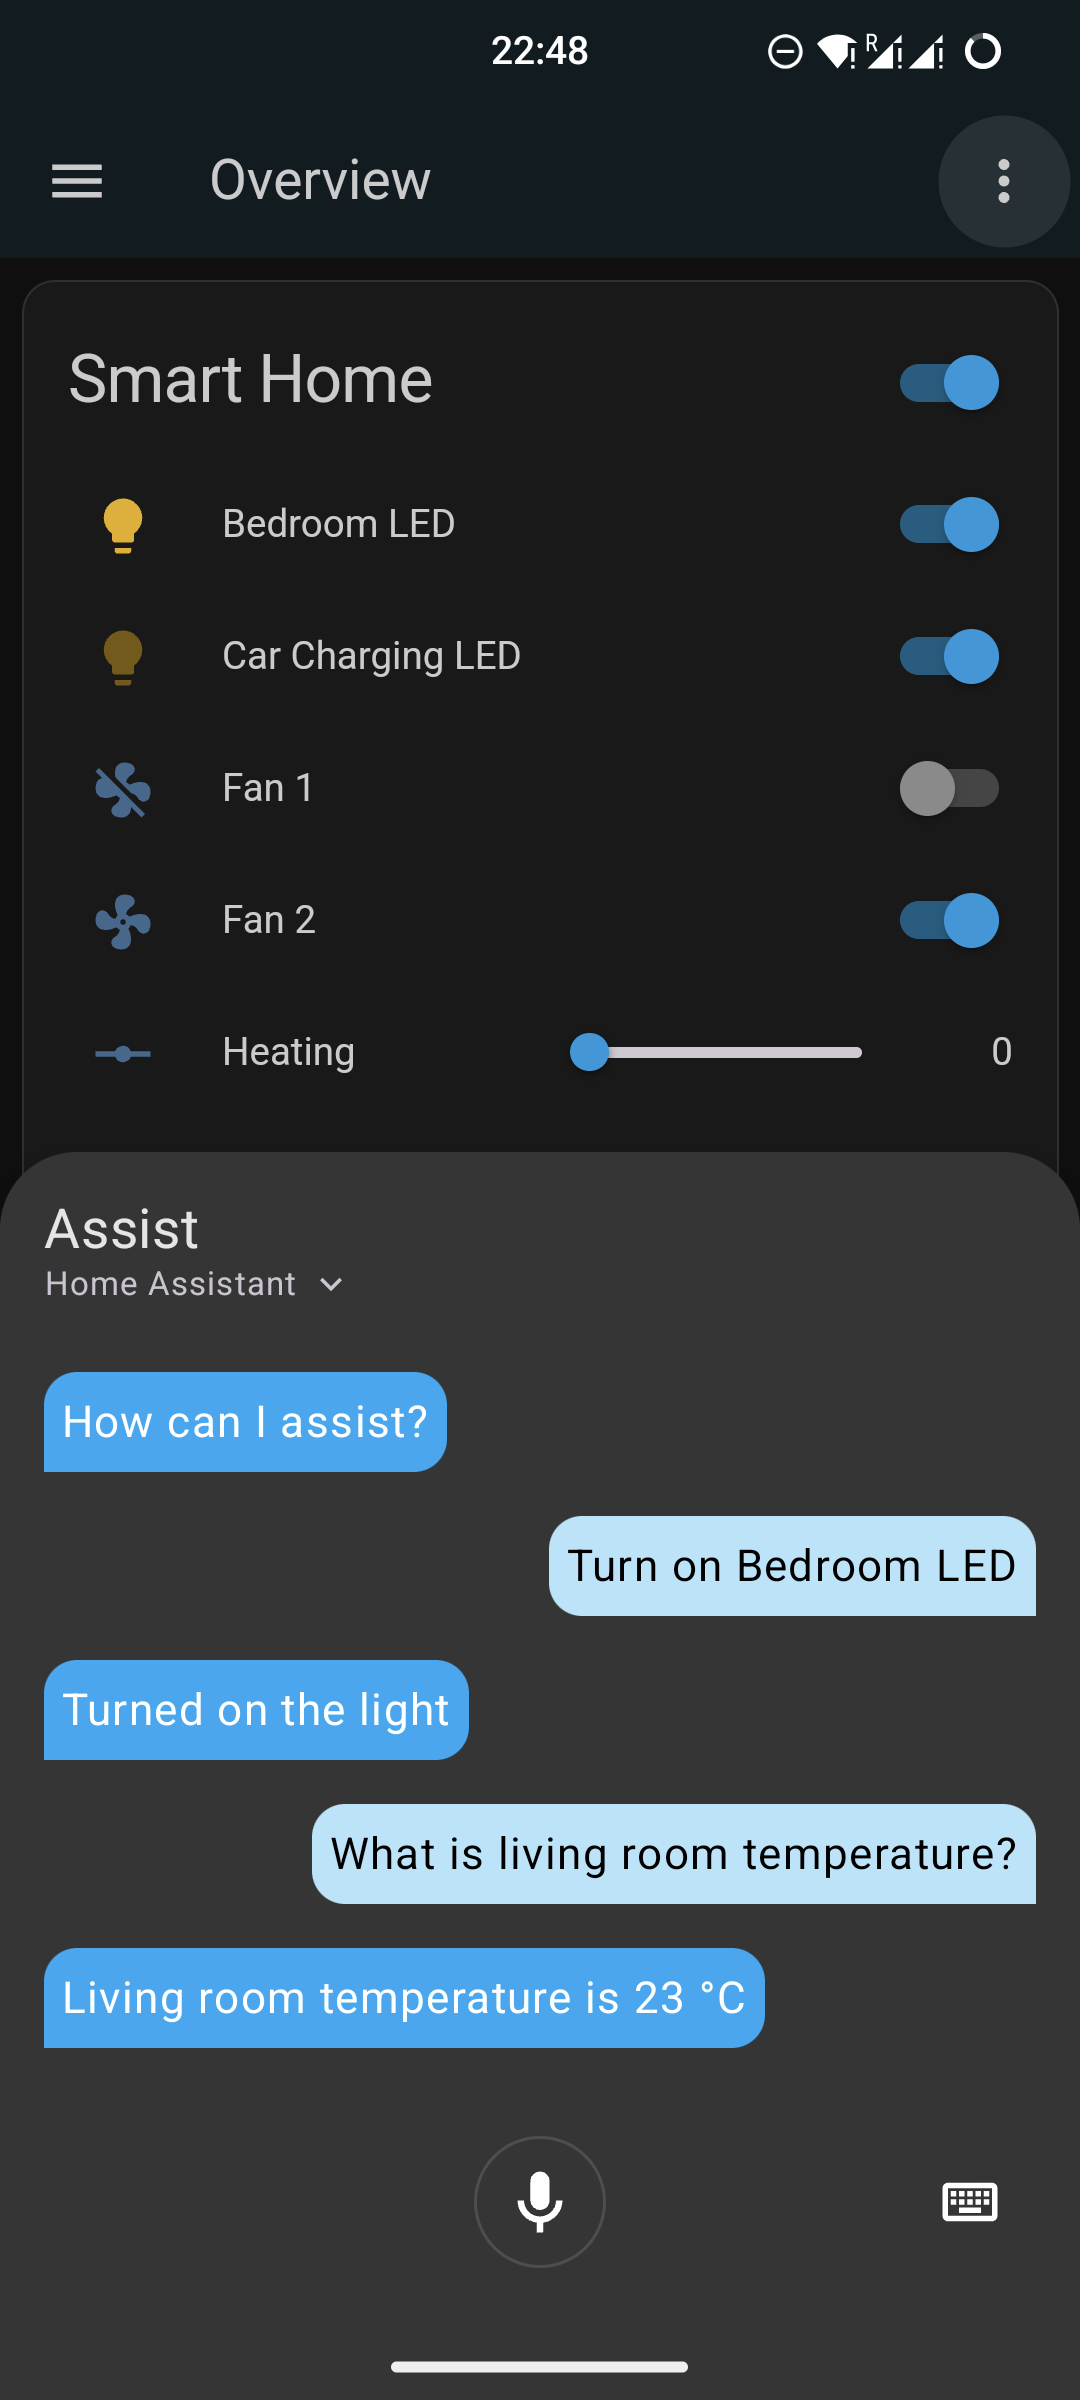
\includegraphics[width=68mm, keepaspectratio]{figures/homeassistant_android_assist.png}
  \caption{Screenshot of Home Assistant's locally hosted voice assistant in action}
  \label{fig:HAandroidVoiceAssistant}
\end{figure}

\chapter{Review}

This chapter mainly focuses on the box model's evalution to the requirements specified during the planning phase, shortcomings, how these could potentially be overcome and finally, opportunities of further development.

\section{Usage}

During usage, controlling the model box's components via the user interface is quite impressive, as when components are toggled and values are altered from a laptop or smartphone, the changes made propagate really fast to the model, in a few seconds at most. Besides control, monitoring of the implemented sensors is also reliable, as when influenced externally eg. with more or less heat, light, the change can be seen in the readings of sensors. These values, along with other metrics, actions taken by the user are logged and this history can be reviewed later, or even be plotted to a graph in case of quantifiable amounts between certain time ranges.

% todo screenshot of temp/brightness graph

The use cases of the model include the most important aspects of a typical smart home environment: monitoring of temperature and light levels, control of basic utilities in the form of heating and cooling, and lastly, a "smartified" rolling shutter (that would be actuated by hand in a conventional home).

\section{Critical analysis, shortcomings}

The experience of using the model box and its user interface is really similar to what a deployed home environment would be, therefore an adequate way to simulate a real smart home system with certain limitations. The model features a full-fledged smart home software platform, which is used in many installations worldwide. % todo source based on github stars, or that it is one of the most popular open source projects
The number of "devices" (according to Home Assistant's terminology) is less, than in a usual real environment with more heterogeneous devices, but the number components connected to it makes it comparable to that of a basic installation.
There are aspects however, that are usually part of a typical installation, but weren't featured in the model, these are security management and energy monitoring systems (besides the solar power car charging simulation), due to the limited scope and resources of the project. They could be simulated with more components added, but it would have increased the project's cost, it is also possible that an other microcontroller would have been needed due to the limited of ports and the features that these provide (eg. PWM, ADC, DAC) not being enough.

With the selected software platforms and devices, the user has absolute control over their smart home infrastructure and its data. With the proper knowledge, it can be changed, further developed and expanded with additional modules due to its open-source nature. In a typical installation, the smart home platform would be run on an always running computer, server or low-powered microcomputer (eg. Raspberry Pi), along with an uninterrupted power supply (UPS) to prevent data loss and quicker recovery from momentary power disruption, instead of running from a laptop, that always transported to different location. However, the system's operation and management requires basic IT system administration knowledge, that many end-users lack, therefore this solution might not be favorable for them and should utilize easier to set-up, out-of-the-box solutions, or hire a contractor, who is specialized in smart home system installations and maintenance.

The smart home platform, its network communication medium and connected devices, appliances should function realiably. If this is not the case and one or more utilities aren't available, their unavailability will cause different levels of inconvenience to the inhabitants of the house. This can range from minor sensor readings not available or updated, to lights or hot water for shower not available, to the lack of heating during winter or air conditioning during summer.

A smart home platform should also have adequate security measures, as its security is only as strong as it's weakest link. The demo box uses a separated Wi-Fi network with a decent pre-shared-key (password) and encryption (WPA2), and the control server is only accessible from this Wi-Fi network or the development laptop and requires authentication with custom credentials set. It is not accessible from the Internet (it is behind Network Address Translation), but a typical environment would be set up for access, therefore security is even more important in that case. If such systems are hacked into, it can have varying negative consequences to their owners: starting from toggling and changing values of appliances, gatewaying into the home network via a compromised device to find additional vulnerabilities, to theft of data and spying in the form of video or audio means (if a camera or voice assistant system is installed). Therefore it is crucial to ensure security, software updates should be installed regularly (and these shouldn't introduce other vulnerabilities or bugs, as it sometimes happens by some irresponsible manufacturers).

The model box's hardware doesn't suffer from vendor lock-in, as it often is in case of many commercial smart home solutions. The platform is modular, parts can be substituted, added and further developed thanks to its open-source property. However, changing the software platforms can be tedious and time-consuming, as the environments need to be set up again and customized to the specific needs and can take between hours to days in a typical home installation.

\section{Opportunities of further development}

more automations, devices

set it up in a real house

add energy, security systems

use z-wave, zigbee, matter devices

develop software, hardware for it as a business

protocol development, iot opportunities

business potential



% Acknowledgements
%~~~~~~~~~~~~~~~~~~~~~~~~~~~~~~~~~~~~~~~~~~~~~~~~~~~~~~~~~~~~~~~~~~~~~~~~~~~~~~~~~~~~~~
%----------------------------------------------------------------------------
\chapter*{\koszonetnyilvanitas}\addcontentsline{toc}{chapter}{\koszonetnyilvanitas}
%----------------------------------------------------------------------------

Ez nem kötelező, akár törölhető is. Ha a szerző szükségét érzi, itt lehet köszönetet nyilvánítani azoknak, akik hozzájárultak munkájukkal ahhoz, hogy a hallgató a szakdolgozatban vagy diplomamunkában leírt feladatokat sikeresen elvégezze. A konzulensnek való köszönetnyilvánítás sem kötelező, a konzulensnek hivatalosan is dolga, hogy a hallgatót konzultálja.


% List of Figures, Tables
%~~~~~~~~~~~~~~~~~~~~~~~~~~~~~~~~~~~~~~~~~~~~~~~~~~~~~~~~~~~~~~~~~~~~~~~~~~~~~~~~~~~~~~
%\listoffigures\addcontentsline{toc}{chapter}{\listfigurename}
%\listoftables\addcontentsline{toc}{chapter}{\listtablename}


% Bibliography
%~~~~~~~~~~~~~~~~~~~~~~~~~~~~~~~~~~~~~~~~~~~~~~~~~~~~~~~~~~~~~~~~~~~~~~~~~~~~~~~~~~~~~~
\bibliography{bib/mybib}
\addcontentsline{toc}{chapter}{\bibname}


% Appendix
%~~~~~~~~~~~~~~~~~~~~~~~~~~~~~~~~~~~~~~~~~~~~~~~~~~~~~~~~~~~~~~~~~~~~~~~~~~~~~~~~~~~~~~
% %----------------------------------------------------------------------------
\appendix
%----------------------------------------------------------------------------
\chapter*{\fuggelek}\addcontentsline{toc}{chapter}{\fuggelek}
\setcounter{chapter}{\appendixnumber}
%\setcounter{equation}{0} % a fofejezet-szamlalo az angol ABC 6. betuje (F) lesz
\numberwithin{equation}{section}
\numberwithin{figure}{section}
\numberwithin{lstlisting}{section}
%\numberwithin{tabular}{section}

%----------------------------------------------------------------------------
\section{A TeXstudio felülete}
%----------------------------------------------------------------------------
\begin{figure}[!ht]
\centering
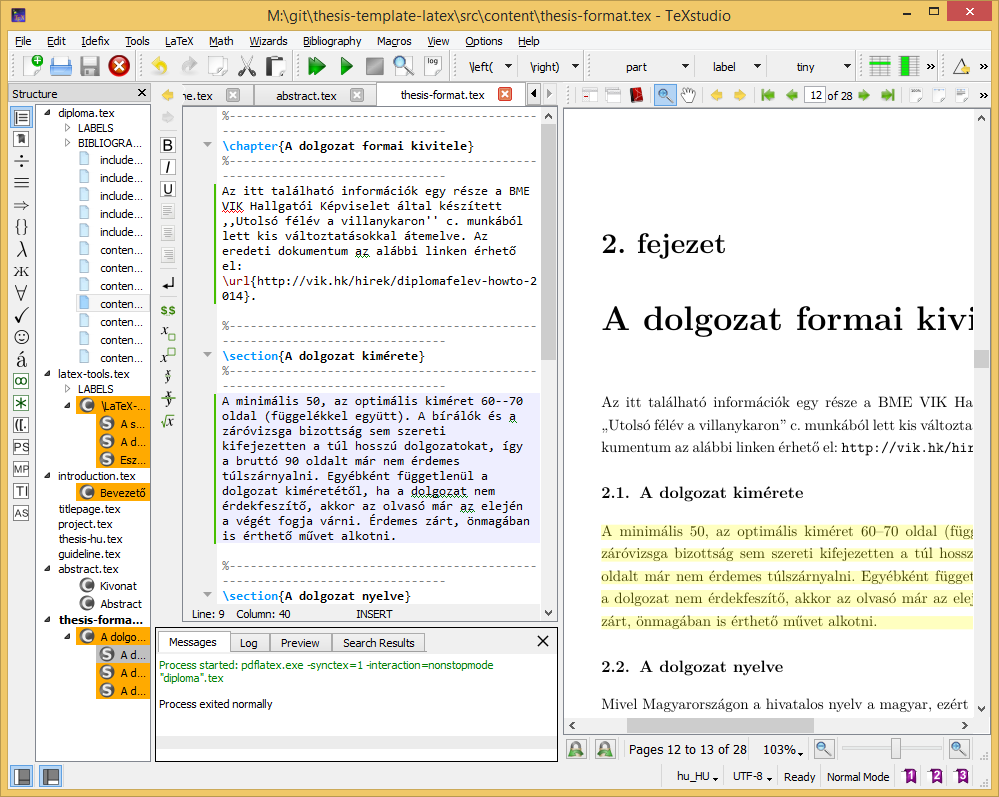
\includegraphics[width=150mm, keepaspectratio]{figures/TeXstudio.png}
\caption{A TeXstudio \LaTeX-szerkesztő.} 
\end{figure}

%----------------------------------------------------------------------------
\clearpage\section{Válasz az ,,Élet, a világmindenség, meg minden'' kérdésére}
%----------------------------------------------------------------------------
A Pitagorasz-tételből levezetve
\begin{align}
c^2=a^2+b^2=42.
\end{align}
A Faraday-indukciós törvényből levezetve
\begin{align}
\rot E=-\frac{dB}{dt}\hspace{1cm}\longrightarrow \hspace{1cm}
U_i=\oint\limits_\mathbf{L}{\mathbf{E}\mathbf{dl}}=-\frac{d}{dt}\int\limits_A{\mathbf{B}\mathbf{da}}=42.
\end{align}


%\label{page:last}
\end{document}
